\documentclass[phd,centertitles,oneside,proposal]{ppgccufmg}
%\documentclass[msc,centertitles,oneside]{ppgccufmg}

\usepackage[english]{babel}      % se o documento for em português, OU

\usepackage[T1]{fontenc}
\usepackage[utf8]{inputenc}

% \usepackage[latin1]{inputenc}
% \inputencoding{latin1}

\usepackage[skins]{tcolorbox}

\usepackage{type1ec}
\usepackage{graphicx}
\usepackage{caption}
\usepackage[labelformat=simple]{subcaption}
\usepackage{longtable}
\usepackage{booktabs}
\usepackage{amsfonts}
\usepackage{units}
\usepackage{enumerate}
\usepackage{multirow,colortbl}
\usepackage[english,
  bookmarks=true,
  bookmarksnumbered=true,
  linktocpage,
  colorlinks,
  citecolor=purple,
  urlcolor=teal,
  linkcolor=blue,
  filecolor=black,
  ]{hyperref}
\usepackage[square,sort,comma,numbers]{natbib}
\newsubfloat{figure}
\usepackage{lettrine} 
\usepackage{tikz}
\usepackage{ctable}
\usepackage[Algoritmo]{algorithm}
\usepackage{algpseudocode}
\usepackage{amssymb}
\usepackage{amsmath}
\usepackage{mathtools}
\usepackage{setspace}
% \usepackage{subfigure}
\usepackage[colorinlistoftodos]{todonotes}
% exemplo de uso
% \todo[inline, color=green!40]{commparação entre segmentação manual e automatica \cite{Swiston2009}}
\usepackage{acro}
\usepackage{threeparttable}
\usepackage{amsmath}
\usepackage{pdflscape}
\usepackage{afterpage}
\usepackage{amsmath,bm}
\usepackage[normalem]{ulem}
\usepackage{bibentry}
\useunder{\uline}{\ul}{}

\newcommand{\novo}[1]{\textcolor{blue}{#1}}
\newcommand{\tirar}[1]{\textit{\textcolor{red}{\sout{#1}}}}
\newcommand{\trocar}[2]{\tirar{#1}\novo{#2}}
\newcommand{\observar}[1]{{\textcolor{violet}{\textbf{\large \uppercase{(#1)}}}}}

\DeclareMathOperator*{\argmax}{arg\,max}
\DeclareMathOperator*{\argmin}{arg\,min}
\DeclareMathOperator*{\sign}{sign}

% Declaracoes em Português
\algrenewcommand\algorithmicend{\textbf{fim}}
\algrenewcommand\algorithmicdo{\textbf{faça}}
\algrenewcommand\algorithmicwhile{\textbf{enquanto}}
\algrenewcommand\algorithmicfor{\textbf{para}}
\algrenewcommand\algorithmicif{\textbf{se}}
\algrenewcommand\algorithmicthen{\textbf{então}}
\algrenewcommand\algorithmicelse{\textbf{senão}}
\algrenewcommand\algorithmicreturn{\textbf{devolve}}
\algrenewcommand\algorithmicfunction{\textbf{função}}

% Rearranja os finais de cada estrutura
\algrenewtext{EndWhile}{\algorithmicend\ \algorithmicwhile}
\algrenewtext{EndFor}{\algorithmicend\ \algorithmicfor}
\algrenewtext{EndIf}{\algorithmicend\ \algorithmicif}
\algrenewtext{EndFunction}{\algorithmicend\ \algorithmicfunction}

% O comando For, a seguir, retorna 'para #1 -- #2 até #3 faça'
\algnewcommand\algorithmicto{\textbf{até}}
\algrenewtext{For}[3]%
{\algorithmicfor\ #1 $\gets$ #2 \algorithmicto\ #3 \algorithmicdo}

% GLOSSARIO
% % GLOSSARIO
% probably a good idea for the nomenclature entries:
\acsetup{first-style=short}

% class `abbrev': abbreviations:
\DeclareAcronym{LSTM}{
  short = LSTM,
  long  = \textit{Long Short-Term Memory},
  class = abbrev
}

\DeclareAcronym{ReLu}{
  short = ReLu,
  long  = \textit{Rectified Linear Unit},
  class = abbrev
}

\DeclareAcronym{ILSVRC}{
  short = ILSVRC,
  long  = \textit{ImageNet Large-Scale Visual Recognition Challenge},
  class = abbrev
}

\DeclareAcronym{GPU}{
  short = GPU,
  long  = \textit{Graphics Processing Unit},
  class = abbrev
}

\DeclareAcronym{ResNet}{
  short = ResNet,
  long  = \textit{Residual Networks},
  class = abbrev
}

\DeclareAcronym{RNN}{
  short = RNN,
  long  = \textit{Recurrent Neural Networks},
  class = abbrev
}

\DeclareAcronym{SGD}{
  short = SGD,
  long  = \textit{Stochastic Gradient Descent},
  class = abbrev
}

\DeclareAcronym{SSD}{
  short = SSD,
  long  = \textit{Single Shot Detector},
  class = abbrev
}

\DeclareAcronym{YOLO}{
  short = YOLO,
  long  = \textit{You Only Look Once},
  class = abbrev
}

\DeclareAcronym{RPN}{
  short = RPN,
  long  = \textit{Region Proposal Network},
  class = abbrev
}

\DeclareAcronym{R-CNN}{
  short = R-CNN,
  long  = \textit{Region-based Convolutional Neural Network},
  class = abbrev
}

\DeclareAcronym{FPS}{
  short = FPS,
  long  = \textit{Frames per Second},
  class = abbrev
}

\DeclareAcronym{mAP}{
  short = mAP,
  long  = \textit{Mean Average Precision},
  class = abbrev
}

\DeclareAcronym{ScSPM}{
  short = ScSPM,
  long  = \textit{Sparse Coding Spatial Pyramid Matching},
  class = abbrev
}

\DeclareAcronym{SIFT}{
  short = SIFT,
  long  = \textit{Scale Invariant Feature Transform},
  class = abbrev
}

\DeclareAcronym{cLBP}{
  short = cLBP,
  long  = \textit{Cell Structured Local Binary Patterns},
  class = abbrev
}

\DeclareAcronym{SVM}{
  short = SVM,
  long  = \textit{Support Vector Machine},
  class = abbrev
}

\DeclareAcronym{EVOC}{
  short = EVOC,
  long  = \textit{Ensemble Video Object Cut},
  class = abbrev
}

\DeclareAcronym{IEC}{
  short = IEC,
  long  = \textit{Iterative Embedded Graph Cut},
  class = abbrev
}

\DeclareAcronym{HOG}{
  short = HOG,
  long  = \textit{Histogram of Oriented Gradient},
  class = abbrev
}

\usepackage{ntheorem}
\newtheorem*{defi_silaba}{Sílaba}
\newtheorem*{defi_chamada}{Chamada}
\newtheorem{mydef}{Defini\c{c}\~ao}

\newcommand{\letracapitular}[1]{\lettrine[lines=3, nindent=0em, slope=-.15em]{\textbf{#1}}{}}

\addto\extrasbrazil{
\let\subsectionautorefname\sectionautorefname 
\let\subsubsectionautorefname\sectionautorefname}

\pdfsuppresswarningpagegroup=1
\pdfminorversion=7

% Fix overfull \vbox on every page: text height exceeds available space by one \baselineskip
\setlength{\textheight}{\textheight}
\addtolength{\textheight}{-\baselineskip}
\checkandfixthelayout[fixed]

\begin{document}

\ppgccufmg{
title={Enhancing Biodiversity Monitoring with Multimodal AI Models for Automated Camera Trap Workflows},
  authorrev={de Alencar, Luiz Fabio Bailosa},
%  cutter={D1234p},
%  cdu={519.6*82.10},
  university={Universidade Federal do Amazonas},
  course={Informática},
  address={Manaus - AM},
  date={2026-07},
  keywords={Redes Neurais Profundas, Armadilhas Fotográficas, Aprendizagem de 
  	Máquina, Transferência de Aprendizado, Monitoramento da Vida Selvagem},
  advisor={Eulanda Miranda dos Santos},
%  approval={img/approvalsheet.eps},
   abstract={Resumo}{resumo},
   abstract=[english]{Abstract}{abstract},
%  dedication={dedicatoria},
%  ack={agradecimentos},
%  epigraphtext={Parecia um aparelho absurdamente complicado, e esse era 
% um dos motivos pelos quais a capa plástica do dispositivo trazia a frase 
% NÃO ENTRE EM PÂNICO em letras grandes e amigáveis.}{O Guia do Mochileiro das 
% Galáxias},
%    beforetoc={\chapter[Lista de Abreviaturas e Siglas]{\centering Lista de 
% Abreviaturas e Siglas} \printacronyms[include-classes=abbrev, heading=none]},
}

\chapter[Introduction]{Introduction}
Wildlife monitoring is a key information source for ecologists and biologists, underpinning a broad array of research in wildlife ecology. It aids in revealing the complex dynamics within ecosystems, assessing the effects of human activities and climate change, and informing effective species conservation measures~\citep{ahumada2013monitoring, he2016visual, tuia2022perspectives, bruce2025large, lindenmayer2022we}. Data collection for these purposes can employ a range of sensors~\citep{tuia2022perspectives}, providing multiple perspectives on animal populations. Examples include remote sensing (satellite or drone images, GPS tags), fixed devices (camera traps and bioacoustic recorders), and citizen-science platforms where members of the public submit observations via systems such as iNaturalist~\citep{horn2018inat, shepley2021automated, herrera2025inaturalist} and eButterfly~\citep{prudic2017ebutterfly}.

\section{Context and motivation}

Camera traps are established, non-invasive, and cost-effective tools for recording wildlife in situ. The data they produce support ecological analyses of terrestrial vertebrate communities, including studies of species occupancy, diversity, abundance, density, community composition, and behavior~\citep{ahumada2013monitoring, beery2021iwildcam, tanwar2021camera, delisle2021next}. These devices are typically triggered by motion or programmed to capture images at scheduled intervals, producing short image or video sequences~\citep{he2016visual}. As a result, camera-trap deployments often generate datasets at a scale that is difficult to process manually. For example, the Snapshot Serengeti project collected 3.2 million images between June 2010 and May 2013 across six seasons~\citep{swanson2015snapshot}, and this collection has since grown to 7.1 million images over eleven seasons~\citep{ss_lila}. Similarly, the Caltech Camera Traps dataset contains 243,100 images from 140 camera locations in the Southwestern United States, annotated across 21 animal categories plus empty images, with approximately 66,000 bounding box annotations. Around 70\% of its images are labeled as empty~\citep{beery2018recognition}. The annotation burden grows with this scale. The original Snapshot Serengeti labeling effort required more than 17,000 volunteer hours~\citep{norouzzadeh2018automatically}, and mobilizing comparable effort is often impractical for smaller studies or for projects focused on less charismatic species.

Over the last decade, deep learning has become a central approach for image analysis and has been widely applied to automate camera-trap data processing. Representative applications include empty-image filtering~\citep{mononen2025active, yousif2019animal, yang2024systematic, cunha2021filtering}, species classification~\citep{chen2023applying, velez2023evaluation, beery2018recognition, norouzzadeh2018automatically}, individual counting~\citep{norouzzadeh2018automatically, norouzzadeh2021deep, arshad2020my, wang2022deep}, and behavior recognition~\citep{schindler2021identification, bain2021automated, binta2023animal, lu2023mammalclub}. In parallel, several software platforms have emerged to help researchers accelerate labeling and information extraction with deep-learning models~\citep{velez2023evaluation}. Some provide user-friendly interfaces that allow a wider community of camera-trap users to train custom models. For example, MegaDetector~\citep{beery2019efficient} is a general detector for animals, people, and vehicles that helps identify relevant frames. The MLWIC2 package provides pre-trained models and training tools for species classification and empty-frame filtering in R~\citep{tabak2020improving}. Other GUI-based platforms, such as Wildlife Insights, Conservation AI, IFLA, and Animal Scanner, have also been developed to simplify information extraction from camera-trap images~\citep{ahumada2020wildlife, chalmers2019conservation, xi2021image, yousif2019animal}.

These AI-driven tools have increased the speed and scalability of camera-trap data processing and annotation, enabling applications at larger scales~\citep{fennell2022use, clarfeld2023evaluating, bohner2023semi, lonsinger2024efficacy}. Recent studies further show the use of these tools in broader and more diverse ecological settings~\citep{celis2024versatile, chen2024minimizing}. Species labels produced by computer-vision models can approximate expert-derived ecological metrics, such as species richness, occupancy, and activity patterns~\citep{whytock2021robust, pantazis2024deep}. Nonetheless, important obstacles persist, including class imbalance and limited generalization across domains~\citep{beery2021scaling, yang2021systematic, zhu2022class, malik2021two}. These limitations are also reported in studies of cross-domain camera-trap recognition~\citep{cunha2023bag}. Moreover, a large portion of camera-trap data still relies on manual processing, which limits the scalability of biodiversity monitoring because of the human labor involved~\citep{beery2023wild}.

\section{Challenges in computer vision for camera-trap data analysis}

Extracting relevant information from camera-trap images involves several difficulties that can hinder accurate analysis, even for experienced specialists. Common problems reported in the literature include animals appearing far from the camera, natural camouflage, complex or unusual body postures, and inadequate lighting conditions~\citep{villa2017towards, norouzzadeh2018automatically, beery2018recognition, gomez2016animal}. Under such circumstances, capturing multiple images per trigger event can improve identification accuracy, as different poses may reveal distinctive morphological features needed for species recognition~\citep{beery2018recognition}.

Domain generalization is another key challenge. Because camera traps are stationary, models can inadvertently learn correlations with site-specific backgrounds present in the training data. This can reduce performance when models are deployed in new environments~\citep{beery2018recognition, schneider2020three, tabak2019machine, norman2023can}.

Beyond these aspects, camera-trap datasets often contain additional complexities, including annotation errors, temporal and spatial dependencies among observations, and limited dataset sizes~\citep{norouzzadeh2018automatically, schneider2020three, brookes2025panaf, bevan2025deep}. Collectively, these challenges motivate methodological approaches that are better aligned with the characteristics of wildlife monitoring data.

\section{Computer vision tasks in automated analysis of camera-trap data}

Before ecologists can incorporate camera-trap data into ecological models, raw images must be processed to extract the information required by the study. This information may include which species are present, how many individuals of each species appear in a capture event, the sex or age class of the animals, and their observed behaviors, such as feeding, resting, or fighting~\citep{norouzzadeh2018automatically}. The required outputs depend on the research question or project goals, and these processing steps can be formulated as computer-vision problems that motivate tailored methods.

A widely investigated task is species recognition, usually formulated as a visual classification problem in which each image is treated as an independent example. Although classification is a classical problem in computer vision, camera-trap datasets introduce several difficulties, including class imbalance~\citep{schneider2020three, johnson2019survey, li2024deep}, few-shot learning scenarios~\citep{alencar2024zero}, and fine-grained distinctions between visually similar species~\citep{van2017devil}. When species-level identification is not possible, labels at higher taxonomic ranks can still have ecological value~\citep{schneider2024recognition}, which introduces an additional hierarchical dimension to the classification problem. Related objectives, such as estimating age, determining sex, and recognizing activities, can also be formulated as classification tasks~\citep{norouzzadeh2018automatically}.

Because many deployments capture multiple images per trigger event to increase the chance of obtaining an informative view, another important problem is species identification using all images from a single capture event~\citep{beery2018recognition, sundaresan2025adapting}. Standard workflows often treat each photo independently during both training and inference. However, exploiting the full image sequence can improve classification when discriminative markings or poses appear only in some frames. In this setting, the goal is to infer species identity from the complete sequence associated with a capture event rather than from a single image.

Given that many camera-trap frames are empty because of incidental sensor activations, automating the removal of empty images is also a practical task. Tools such as MegaDetector have been widely used for this purpose~\citep{beery2019efficient, gadot2024crop, velez2023evaluation, leorna2022human}. Empty-image filtering reduces the amount of data that must be reviewed manually and can serve as an initial step before downstream tasks such as species classification and behavior recognition.

\section{Research Hypotheses}

This thesis is guided by three hypotheses concerning the use of multimodal pre-trained models in camera-trap workflows under limited supervision.

\begin{description}
  \item[H1] Pre-trained multimodal models can support core camera-trap tasks, including empty-image filtering, species classification, and behavior identification, under zero-shot and few-shot settings without requiring task-specific training for each task.

  \item[H2] In zero-shot species classification, combining visual similarity with textual similarity can improve top-1 accuracy relative to a visual-only baseline, although the magnitude of the improvement may depend on the dataset and image setting.

  \item[H3] A low-supervision multimodal approach can provide empirical evidence for reducing dependence on annotated camera-trap data while identifying the conditions under which multimodal models and visual-textual fusion are most useful for biodiversity monitoring workflows.
\end{description}

\section{Objectives}

\subsection{General Objective}

To investigate the conditions under which multimodal machine learning models can support and improve the automation of camera-trap workflows for biodiversity monitoring, with emphasis on ecological vision tasks under low-supervision and zero-shot settings.

\subsection{Specific Objectives}

\begin{description}

\item[1.] To evaluate the potential of multimodal foundation models for core camera-trap tasks, including empty-image filtering, species classification, and behavior identification.

\item[2.] To assess how the performance of multimodal models varies across task types, supervision regimes, and input contexts in camera-trap data.

\item[3.] To propose and evaluate a zero-shot multimodal fusion strategy for species classification based on the integration of visual similarity and textual similarity.

\item[4.] To analyze the conditions and limitations that affect the effectiveness of multimodal models and visual-textual fusion in camera-trap workflows.

\item[5.] To synthesize the empirical findings and proposed methods into a final contribution that clarifies when and how multimodal models can reduce dependence on task-specific training and annotated camera-trap data.

\end{description}

\subsection{Intended Contributions}

The intended contributions of this thesis are as follows:

\begin{itemize}

\item An empirical evaluation of multimodal foundation models for multiple stages of the camera-trap workflow, covering empty-image filtering, species classification, and behavior identification.

\item An analysis of multimodal model behavior under low-supervision scenarios, including zero-shot and few-shot settings and, for behavior identification, the use of image sequences.

\item A zero-shot multimodal fusion strategy for species classification that combines CLIP-based visual similarity with language-model-assisted textual similarity.

\item Evidence on the conditions under which multimodal models and visual-textual fusion can improve camera-trap analysis, as well as the cases in which these approaches remain limited.

\item A methodological basis for reducing dependence on large annotated datasets in camera-trap workflows while preserving practical relevance for biodiversity monitoring.

\end{itemize}

\section{Organization of the Document}

The remainder of this thesis is organized as follows. Chapter 2 presents the fundamental concepts required to understand the work, including zero-shot and few-shot learning, multimodal large language models, image preprocessing, training techniques, and evaluation metrics. Chapter 3 reviews related work on automated camera-trap analysis, focusing on empty-image filtering, species recognition, behavior recognition, multimodal learning, and fusion-based approaches. Chapter 4 presents the first empirical study, which evaluates multimodal models in three camera-trap tasks: empty-image filtering, species classification, and behavior identification. Chapter 5 presents the proposed multimodal fusion strategy for zero-shot species classification and evaluates it across different datasets and image settings. Finally, Chapter 6 summarizes the thesis contributions and outlines the next steps and schedule for completing the research.
\chapter{Fundamentals}\label{cap:fundamentals}

This chapter introduces the fundamental concepts that underpin this work. We begin with an overview of key machine learning topics relevant to our study, including computer vision architectures, multimodal large language models, image preprocessing methods, training strategies, and evaluation metrics. We then examine the main challenges and limitations associated with these approaches, situating them within the broader context of our research.

Finally, we summarize the core ideas discussed in this chapter and explain how they connect to the remainder of the thesis. Overall, this chapter provides the conceptual and technical foundation necessary to understand the methods and results presented in the subsequent chapters, particularly for readers who may not be familiar with the underlying principles of machine learning and computer vision.


\section{Computer vision architectures}

\section{Multimodal Large Language Models}
\subsection{CLIP}

Contrastive Language-Image Pre-training (CLIP), introduced by ~\citep{radford2021learning}, proposes a departure from traditional supervised computer vision by replacing fixed, manually annotated label sets with large-scale natural language supervision. Instead of training a model to predict one among a predefined list of categories, CLIP learns directly from approximately 400 million image-text pairs collected from the internet. The central intuition is that natural language offers a far richer and more flexible supervisory signal than curated taxonomies such as ImageNet classes. Text descriptions associated with images encode not only object names, but attributes, relationships, actions, and contextual cues. By leveraging this weak but abundant supervision at web scale, CLIP aims to learn visual representations that are inherently aligned with language and therefore more transferable across tasks and domains.

Technically, CLIP is composed of two neural networks trained jointly: an image encoder (either a modified ResNet or a Vision Transformer) and a Transformer-based text encoder (see Figure
\ref{fig:clip_architecture}). Each encoder maps its input into a latent vector space, and both outputs are projected into a shared multimodal embedding space where cosine similarity measures semantic alignment. Rather than generating captions or predicting words token by token, CLIP uses a contrastive objective: given a minibatch of $(N)$ image-text pairs, the model learns to identify the correct pairing among all $(N^2)$ possible combinations. The training objective maximizes similarity between matched pairs and minimizes similarity between mismatched ones using a symmetric cross-entropy loss over temperature-scaled cosine similarities. This formulation significantly improves training efficiency compared to generative captioning approaches and enables stable large-scale training from scratch without pre-initialization from supervised models.

\begin{figure*}[!ht]
\centering
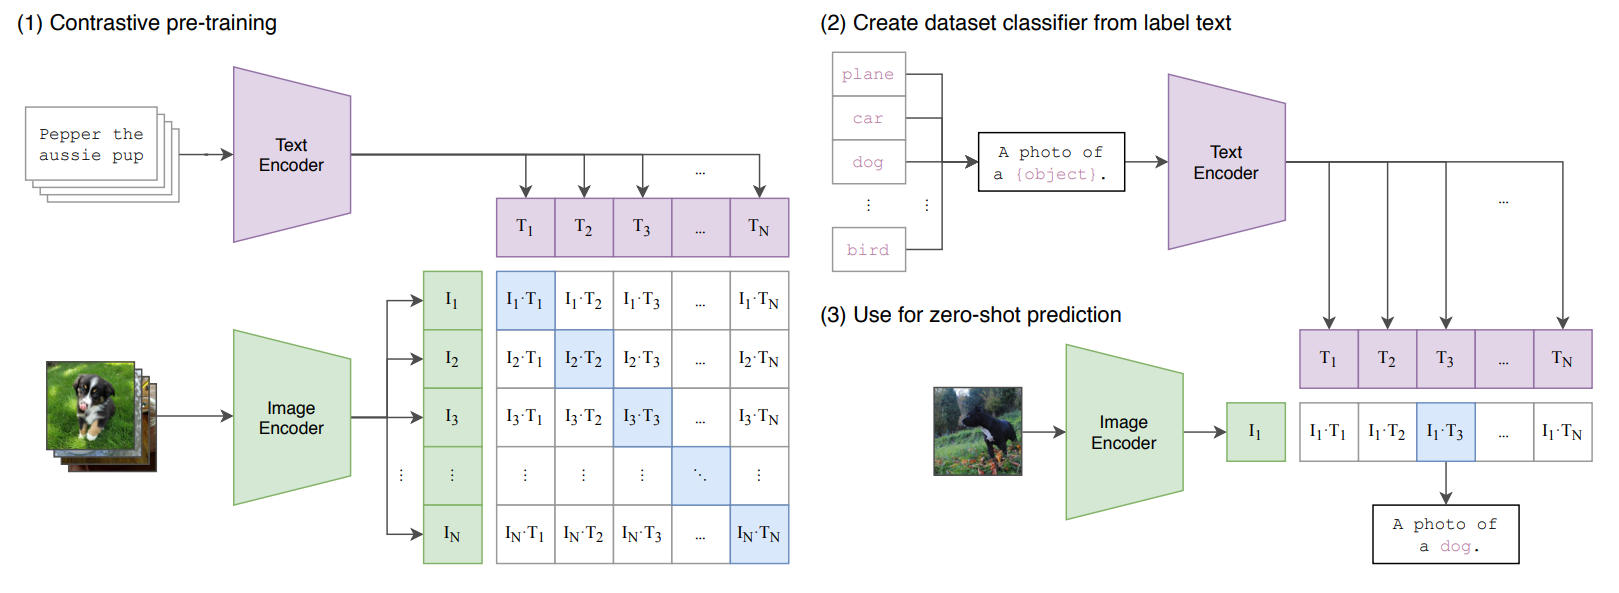
\includegraphics[width=6in]{images/clip.png}
\caption{CLIP architecture}
\legend{Source: \citet{radford2021learning}.}
\label{fig:clip_architecture}
\end{figure*}

A defining property of CLIP is its ability to perform zero-shot transfer. Because the model learns a joint embedding space aligned with natural language, it can be adapted to a new classification task without additional training. To classify images in a new dataset, one simply encodes textual prompts describing each class (e.g., “a photo of a dog”), embeds them using the text encoder, and compares them to image embeddings via cosine similarity . This effectively produces a linear classifier whose weights are dynamically generated from language. In zero-shot evaluation on ImageNet, CLIP achieves 76.2\% top-1 accuracy, matching the original supervised ResNet-50 despite using none of ImageNet's labeled training examples ~\citep{radford2021learning}. Across more than 30 datasets covering object recognition, fine-grained classification, action recognition, optical character recognition, and geo-localization, CLIP often performs competitively with fully supervised baselines, and in many cases surpasses linear probes trained on conventional ImageNet features.

Beyond raw performance, CLIP exhibits several notable empirical properties. Its zero-shot performance scales smoothly with model size and compute, following predictable log-log trends similar to those observed in large language models. Larger Vision Transformer variants outperform convolutional counterparts in compute efficiency, and representation learning evaluations show that CLIP features can exceed those of state-of-the-art supervised and self-supervised models on diverse benchmarks. At the same time, the model reveals limitations in tasks requiring fine spatial reasoning, counting, or highly specialized domain knowledge, highlighting that semantic alignment alone does not guarantee structured reasoning capabilities ~\citep{radford2021learning}. Overall, CLIP demonstrates that large-scale multimodal contrastive learning can produce open-vocabulary visual systems with strong generalization ability, establishing a foundation for subsequent multimodal and vision-language models.

\subsection{BLIP}
Bootstrapping Language-Image Pre-training (BLIP) is a vision–language framework designed to improve the performance of multimodal models on both understanding and generation tasks. Traditional vision–language models typically focus on a single category of tasks, such as image–text retrieval or image captioning. BLIP addresses this limitation by proposing a unified architecture capable of supporting a wide range of multimodal tasks. In addition to its architectural design, the framework introduces a data bootstrapping strategy that improves the quality of large-scale image–text datasets collected from the web, which often contain noisy or inaccurate captions ~\citep{li2022blip}. 

The BLIP model is built upon a Multimodal Mixture of Encoder–Decoder (MED) architecture that enables it to operate in multiple modes depending on the task being performed. The architecture combines a visual encoder, typically based on a Vision Transformer (ViT), with a text transformer that processes textual inputs and interacts with visual representations through cross-attention layers (see Figure
\ref{fig:blip_architecture}). This design allows the model to function as a unimodal encoder for representation learning, as an image-grounded text encoder for multimodal understanding, or as an image-grounded text decoder for text generation. As a result, BLIP can effectively learn relationships between visual content and language while also generating natural language descriptions conditioned on images  ~\citep{li2022blip}. 

\begin{figure*}[!ht]
\centering
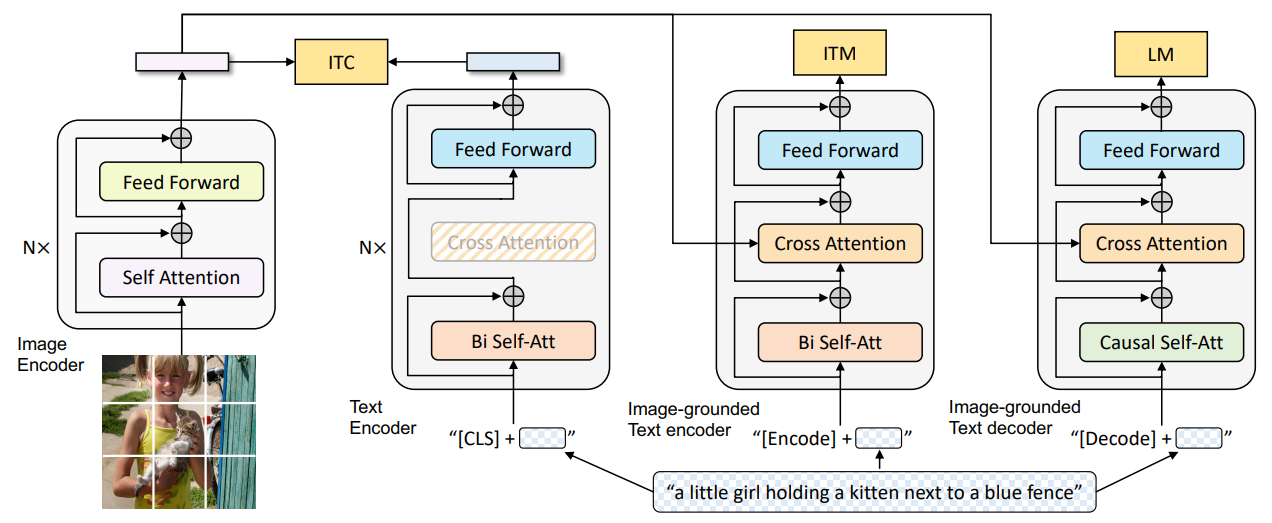
\includegraphics[width=6in]{images/blip.png}
\caption{BLIP architecture}
\legend{Source: \citet{li2022blip}.}
\label{fig:blip_architecture}
\end{figure*}

During pre-training, BLIP optimizes three complementary learning objectives that strengthen the alignment between images and text. The image–text contrastive (ITC) objective aligns visual and textual representations in a shared embedding space, improving retrieval performance. The image–text matching (ITM) objective determines whether a given image and text pair correspond to each other, encouraging the model to capture fine-grained multimodal relationships. Finally, a language modeling (LM) objective allows the model to generate textual descriptions from visual inputs using an autoregressive decoding process. Together, these objectives enable the model to perform both multimodal understanding and generation tasks within a single framework  ~\citep{li2022blip}. 

Another important contribution of BLIP is its Captioning and Filtering (CapFilt) data bootstrapping strategy, which improves the quality of training datasets. Web-collected image–text pairs often contain noisy captions that may not accurately describe the visual content. To address this issue, BLIP employs a captioning model to generate synthetic captions for images and a filtering model to remove low-quality text descriptions. This process produces a cleaner and more informative training dataset, which significantly enhances the model’s performance across several tasks, including image–text retrieval, image captioning, and visual question answering. Experimental results demonstrate that this approach leads to substantial improvements compared to previous vision–language models trained on similar data scales ~\citep{li2022blip}. 

\subsection{GPT}
The Generative Pre-trained Transformer (GPT) is a family of large language models designed to understand and generate natural language text. GPT models are based on the Transformer architecture and are trained using large-scale text corpora to learn statistical patterns in language. Through this training process, the model learns to predict the next token in a sequence given the previous context, enabling it to generate coherent and contextually relevant text. Because of this autoregressive formulation, GPT can perform a wide variety of language tasks without requiring task-specific architectures ~\citep{achiam2023gpt}. 

GPT models rely on a Transformer-based architecture that uses self-attention mechanisms to model relationships between tokens in a sequence. During training, the model processes large amounts of text data and learns representations that capture syntactic, semantic, and contextual information. The model is first trained through a large-scale pretraining phase using unlabeled text data and later refined through post-training techniques such as reinforcement learning with human feedback (RLHF), which aligns the model’s outputs with human preferences and improves instruction-following capabilities ~\citep{achiam2023gpt}. 

Due to their ability to generate and interpret language, GPT models can be applied to a broad range of natural language processing tasks. These include text generation, question answering, summarization, translation, code generation, and conversational agents. More recent versions of the model also support multimodal inputs and can interact with external tools and systems to perform more complex reasoning tasks. In practical applications, GPT models are frequently used in chatbots, educational tools, research assistance, and software development environments ~\citep{achiam2023gpt}. 

Experimental evaluations demonstrate that modern GPT models achieve strong performance across many academic and professional benchmarks (see Figure
\ref{fig:gpt_results}). For instance, GPT-4 has been shown to outperform previous language models on a wide range of tasks and achieve human-level performance on several standardized exams and professional assessments. Results reported in the study indicate that the model performs competitively across multiple domains, including science, mathematics, law, and general knowledge tests, highlighting the broad capabilities of large-scale language models ~\citep{achiam2023gpt}. 

\begin{figure*}[!ht]
\centering
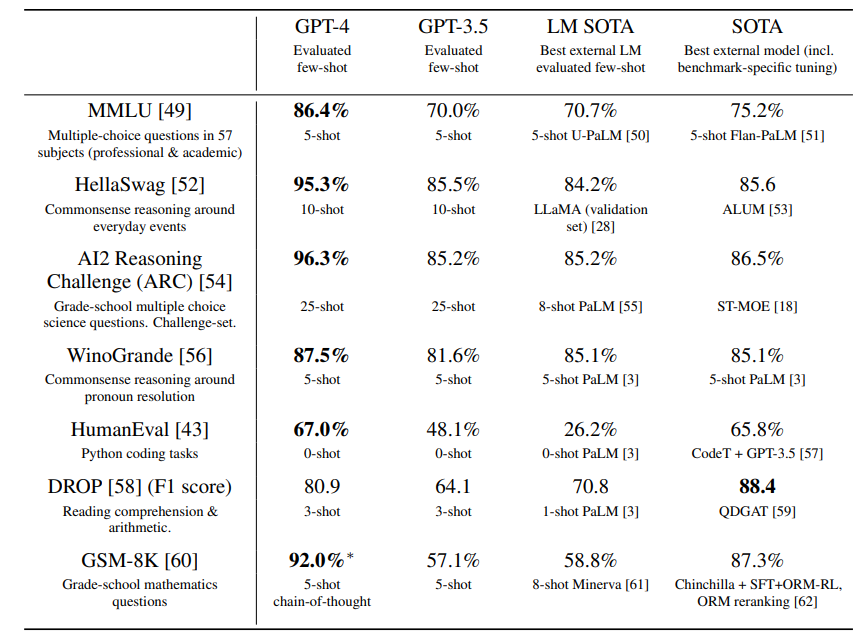
\includegraphics[width=6in]{images/gpt.png}
\caption{Performance of GPT-4 across multiple academic benchmarks as reported by the authors. The results show that GPT-4 consistently outperforms previous language models and achieves competitive performance compared with state-of-the-art systems trained specifically for individual benchmarks, demonstrating strong few-shot learning capabilities across diverse evaluation tasks.}
\legend{Source: \citet{achiam2023gpt}.}
\label{fig:gpt_results}
\end{figure*}

\subsection{Gemini}
Gemini is a family of large multimodal artificial intelligence models developed to advance capabilities in reasoning, language understanding, and cross-modal processing. Unlike traditional language models that primarily operate on text, Gemini was designed from the outset as a natively multimodal system, capable of processing and reasoning over multiple types of data, including text, images, audio, and video \citet{team2023gemini}. The model family includes different variants—Gemini Ultra, Gemini Pro, and Gemini Nano—which are optimized for different levels of computational capability and deployment environments. Ultra represents the most powerful model for complex reasoning and multimodal tasks, Pro is optimized for performance and efficiency across a wide range of applications, and Nano is designed for on-device deployment in resource-constrained environments. 

The architecture of Gemini is based on an enhanced decoder-only Transformer model, incorporating architectural improvements and optimization techniques to enable stable large-scale training. The models support long context windows of up to 32,000 tokens and use efficient attention mechanisms such as multi-query attention to improve computational efficiency. A key innovation of Gemini is its ability to process interleaved multimodal inputs, meaning that text, images, audio signals, and video frames can be provided within the same sequence of tokens (see Figure
\ref{fig:gemini_architecture}). Visual and video information are encoded as sequences of image frames within the context window, while audio signals are represented using features extracted from speech models. This design allows Gemini to perform complex reasoning tasks that require integrating information from multiple modalities within a single unified framework \citet{team2023gemini}. 

\begin{figure*}[!ht]
\centering
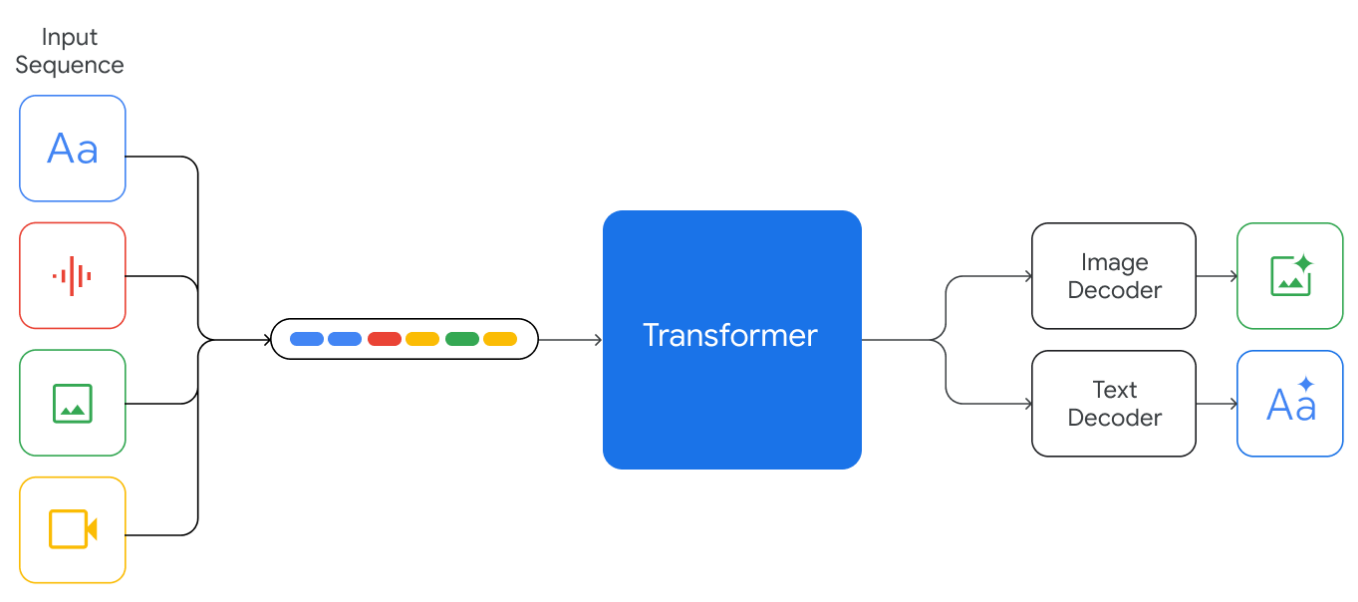
\includegraphics[width=6in]{images/gemini.png}
\caption{Illustration of the multimodal reasoning capabilities of Gemini models. According to the authors, Gemini can process sequences containing interleaved text, images, audio, and video, enabling the model to generate responses that combine textual and visual information within a unified multimodal framework}
\legend{Source: \citet{team2023gemini}.}
\label{fig:gemini_architecture}
\end{figure*}

Gemini models are trained on a large-scale multimodal and multilingual dataset composed of web documents, books, code repositories, images, audio, and video data. The training process involves extensive data filtering and safety mechanisms to ensure quality and remove harmful content. During pre-training, the model learns representations that capture relationships across different modalities, enabling it to perform tasks such as multimodal reasoning, content generation, summarization, and information extraction \citet{team2023gemini}. After pre-training, additional post-training procedures—including instruction tuning and reinforcement learning from human feedback—are applied to improve the model's ability to follow instructions and generate responses aligned with human expectations. 

Experimental results demonstrate that Gemini models achieve state-of-the-art performance across multiple benchmarks, including tasks involving reasoning, mathematics, coding, and multimodal understanding. In particular, Gemini Ultra surpasses human-expert performance on the MMLU benchmark, achieving an accuracy of approximately 90\%, and sets new state-of-the-art results across a wide range of text, image, audio, and video evaluation tasks. The model also shows strong performance in mathematical reasoning benchmarks such as GSM8K and coding benchmarks like HumanEval. These results highlight Gemini's ability to function as a general-purpose multimodal model capable of solving complex problems and enabling applications in areas such as education, software development, accessibility technologies, and intelligent assistants \citet{team2023gemini}.

\section{Image preprocessing techniques}
Image preprocessing is a fundamental step in computer vision pipelines, as raw images often need to be transformed into a standardized format before being used to train machine learning models. These preprocessing operations ensure that the data are compatible with the input requirements of neural network architectures and that the training process remains stable and efficient. Common preprocessing procedures include operations such as image resizing, normalization of pixel values, and data augmentation. Together, these techniques help prepare image datasets for effective learning by reducing variability caused by acquisition conditions while preserving relevant visual information.

One of the most common preprocessing steps is normalization, which consists of scaling the pixel intensity values to a standardized numerical range. Image pixel values are typically represented in the range ([0, 255]), and normalization transforms these values to smaller intervals such as ([0, 1]) or ([-1, 1]). In deep learning pipelines, it is also common to standardize images using the mean and standard deviation computed from the training dataset or from widely used datasets such as ImageNet. This procedure helps stabilize gradient updates during optimization and often accelerates the convergence of training algorithms by ensuring that input features have comparable numerical scales \citep{goodfellow2016deep}.

Another important preprocessing operation is image resizing, which adjusts the spatial resolution of images to match the input dimensions expected by the model architecture \citep{goodfellow2016deep}. Many convolutional neural networks require fixed-size inputs, such as (224 X 224) or (299 X 299) pixels, which makes resizing a necessary step when working with datasets containing images of varying resolutions. Resizing can be performed using interpolation techniques that preserve the overall structure of the visual content while adapting it to the required size. Although some modern architectures are capable of processing images with variable spatial dimensions, resizing remains widely used to standardize inputs and optimize computational efficiency during training and inference.

Data augmentation is another critical preprocessing technique that aims to artificially increase the diversity of the training dataset by applying controlled transformations to existing images (see Figure \ref{fig:data-augmentation}). These transformations may include horizontal or vertical flipping, rotations, random cropping, translations, and adjustments to color properties such as brightness, contrast, and saturation \citep{maharana2022review, shorten2019survey}. By exposing the model to multiple variations of the same image, data augmentation helps reduce overfitting and improves the ability of the model to generalize to unseen data. However, designing an effective augmentation pipeline can be challenging, as the choice of transformations and their parameters must be consistent with the characteristics of the dataset and the target task. Excessive or inappropriate transformations may distort relevant visual features or introduce unrealistic patterns, potentially degrading model performance. Consequently, careful selection and tuning of preprocessing strategies are essential to achieve robust and reliable results in computer vision applications \citep{maharana2022review}.

\begin{figure*}[!ht]
\centering
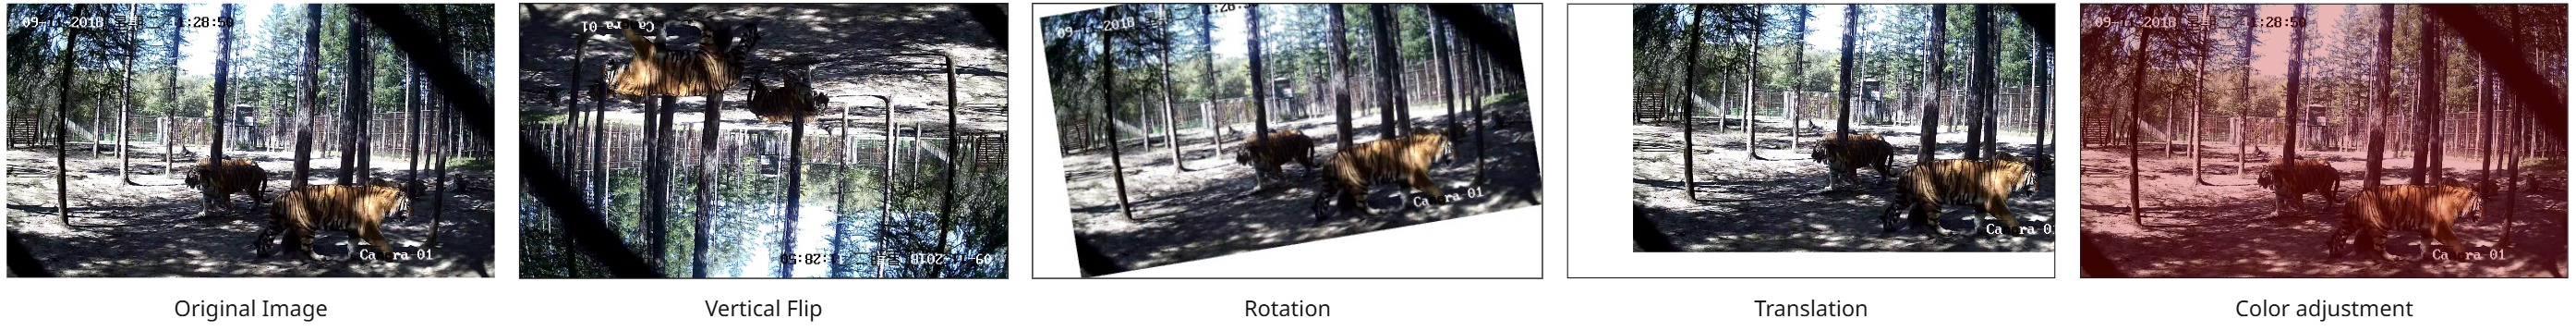
\includegraphics[width=6in]{images/data-augmentation.png}
\caption{Data augmentation examples}
\legend{Source: Author.}
\label{fig:data-augmentation}
\end{figure*}

\section{Training techniques}
The training of deep neural networks represents a high-dimensional, non-convex optimization problem where the objective is to minimize a loss function $\mathcal{L}(\theta)$ relative to a set of parameters $\theta \in \mathbb{R}^d$. This process is not merely a computational exercise in gradient descent but a complex interplay between algorithmic stability, numerical convergence, and the ultimate goal of statistical generalization \cite{goodfellow2016deep}.

\subsection{The Optimization Landscape: SGD vs. Adaptive Methods}

At the core of neural network training is the optimization landscape, a manifold characterized by saddle points, plateaus, and local minima. The choice of optimizer determines how the trajectory of $\theta$ navigates this surface.

\subsubsection{Stochastic Gradient Descent (SGD)}
SGD remains the foundational algorithm, updating parameters via:
\begin{equation}
\theta_{t+1} = \theta_t - \eta \nabla \mathcal{L}(\theta_t; x^{(i)}, y^{(i)})
\end{equation}
where $\eta$ is the learning rate. While computationally efficient, vanilla SGD often struggles with "ravines" where the surface curves much more steeply in one dimension than another. The introduction of momentum mitigates this by accumulating a velocity vector, effectively smoothing the path and accelerating convergence in consistent directions.

\subsubsection{Adaptive Methods: Adam and Beyond}
Adaptive optimizers, most notably Adam (Adaptive Moment Estimation), maintain per-parameter learning rates. Adam computes individual updates based on estimates of the first and second moments of the gradients:
\begin{align}
m_t &= \beta_1 m_{t-1} + (1 - \beta_1)g_t \\
v_t &= \beta_2 v_{t-1} + (1 - \beta_2)g_t^2
\end{align}
While Adam typically exhibits faster initial convergence, empirical evidence suggests that SGD with momentum often leads to better generalization on the test set \cite{wilson2018marginalvalueadaptivegradient}.

\subsection{Dynamic Training Protocols}

Optimization is rarely a static process. To navigate the loss surface effectively, researchers employ dynamic protocols that adjust the training regime in real-time.

\begin{itemize}
    \item \textbf{Learning Rate (LR) Scheduling:} A static $\eta$ is often suboptimal. Early training requires a high $\eta$ to escape local suboptimality, while later stages require a decaying $\eta$ to settle into the global minimum.
    \item \textbf{Early Stopping:} This serves as a temporal regularizer. By monitoring the loss on a disjoint validation set, training is halted once the validation error begins to diverge from the training error, preventing the model from memorizing noise.
\end{itemize}

\subsection{Regularization and the Bias-Variance Tradeoff}

The fundamental challenge in deep learning is the bias-variance tradeoff: balancing the model's ability to fit the training data against its ability to perform on unseen data.

\subsubsection{Weight Decay ($L_2$ Regularization)}
Weight decay modifies the objective function by adding a penalty term proportional to the square of the magnitude of the weights:
\begin{equation}
\mathcal{L}_{reg} = \mathcal{L} + \lambda \sum \theta^2
\end{equation}
This forces the optimization process to prefer smaller weights, resulting in a smoother mapping function.

\subsubsection{Dropout}
Dropout is a stochastic regularization technique where, during each training iteration, a fraction $p$ of neurons is randomly set to zero. This prevents co-adaptation, where neurons rely on the presence of specific other neurons to correct their errors \cite{srivastava2014dropout}.

\subsection{Practical Challenges and Modern Solutions}

\begin{itemize}
    \item \textbf{Vanishing and Exploding Gradients:} In deep networks, backpropagation can cause gradients to vanish or explode. Modern solutions include residual connections (ResNets) and gradient clipping.
    \item \textbf{Internal Covariate Shift:} As parameters change, the distribution of inputs to subsequent layers shifts. Batch Normalization (BN) addresses this by normalizing activations to have zero mean and unit variance within a mini-batch \cite{ioffe2015batch}.
\end{itemize}

\subsection{Mathematical Analysis of Adam's Convergence}

The convergence of Adam is analyzed through Regret Analysis. For a sequence of convex loss functions $f_1, \dots, f_T$, the regret $R(T)$ is bounded by:
\begin{equation}
R(T) = \sum_{t=1}^T [f_t(\theta_t) - f_t(\theta^*)] \leq O(\sqrt{T})
\end{equation}
However, it is critical to note that Adam can fail to converge in specific settings where the effective learning rate increases over time \cite{reddi2019convergenceadam}. The AMSGrad variant addresses this by ensuring $\hat{v}_t = \max(\hat{v}_{t-1}, v_t)$.

\section{Evaluation Metrics}

The rigorous assessment of model performance is a cornerstone of deep learning research. Relying on a single scalar value often fails to capture the nuances of model behavior, particularly in complex high-dimensional feature spaces. This section details the mathematical and conceptual frameworks for evaluating classification performance, with a specific focus on metrics robust to class distribution shifts.

\subsection{Classification Metrics}

Classification performance is typically derived from the \textit{Confusion Matrix}, which partitions predictions into True Positives ($TP$), True Negatives ($TN$), False Positives ($FP$), and False Negatives ($FN$). While these counts provide a raw view of performance, normalized metrics are required for comparative analysis.

\subsubsection{Accuracy}
Accuracy represents the ratio of correctly predicted observations to the total observations:
\begin{equation}
\text{Accuracy} = \frac{TP + TN}{TP + TN + FP + FN}
\end{equation}
Despite its ubiquity, accuracy is notoriously misleading in the presence of \textbf{class imbalance}. In a dataset where 99\% of samples belong to the majority class, a "naive" classifier that always predicts the majority class achieves 99\% accuracy while failing to learn any discriminative features of the minority class.

\subsubsection{Precision, Recall, and the F1-Score}
To address the limitations of accuracy, we employ metrics that isolate the performance on the positive (often minority) class:

\begin{itemize}
    \item \textbf{Precision (Positive Predictive Value):} Measures the fidelity of the model's positive predictions. It is the ratio of correctly predicted positive observations to the total predicted positives.
    \begin{equation}
    \text{Precision} = \frac{TP}{TP + FP}
    \end{equation}
    
    \item \textbf{Recall (Sensitivity):} Measures the model's ability to find all relevant cases within a dataset. 
    \begin{equation}
    \text{Recall} = \frac{TP}{TP + FN}
    \end{equation}
    
    \item \textbf{F1-Score:} The harmonic mean of Precision and Recall. Unlike the arithmetic mean, the harmonic mean penalizes extreme values, ensuring that a high F1-score requires both high precision and high recall.
    \begin{equation}
    F_1 = 2 \cdot \frac{\text{Precision} \cdot \text{Recall}}{\text{Precision} + \text{Recall}}
    \end{equation}
\end{itemize}

In doctoral research, the choice between these depends on the \textbf{cost of error}. In medical diagnosis, high Recall is often prioritized to avoid missing true cases (False Negatives), whereas in spam detection, high Precision is favored to avoid misclassifying legitimate emails (False Positives).

\subsection{Precision-Recall Curve}

In many deep learning architectures, the final layer outputs a probability distribution rather than a discrete label. The conversion to a label depends on a \textit{classification threshold} $\tau$ (conventionally set at 0.5). However, the optimal $\tau$ is rarely static.

\subsubsection{The Threshold Trade-off}
The Precision-Recall (PR) curve is constructed by plotting Precision against Recall at every possible threshold $\tau \in [0, 1]$. As the threshold decreases, the model becomes more "permissive" increasing Recall but typically decreasing Precision as more False Positives are introduced.



\subsubsection{Area Under the Precision-Recall Curve (AUPRC)}
The AUPRC (or Average Precision) provides a single-figure summary of the PR curve:
\begin{equation}
\text{AUPRC} = \sum_{n} (R_n - R_{n-1}) P_n
\end{equation}
where $P_n$ and $R_n$ are the precision and recall at the $n$-th threshold. 

\subsubsection{PR vs. ROC in Imbalanced Scenarios}
While the Receiver Operating Characteristic (ROC) curve is frequently used, it can present an overly optimistic view of model performance when the negative class is overwhelming. This is because the False Positive Rate ($FP / (FP+TN)$) remains small due to the large $TN$ denominator. The PR curve, by contrast, does not include $TN$ in its primary axes, making it a far more sensitive and honest indicator of performance for imbalanced tasks common in anomaly detection and rare-event prediction.

\section{Final Remarks}

This chapter established the theoretical and technical frameworks—ranging from foundational deep learning to multimodal systems such as CLIP, BLIP, and Gemini—necessary for robust wildlife classification. The transition from unimodal computer vision to vision-language models demonstrates how semantic alignment between text and imagery enhances model generalization. Furthermore, the analysis of optimization, regularization, and preprocessing highlights the importance of algorithmic stability when processing high-variance visual data from outdoor environments. The focus on evaluation metrics robust to class imbalance, specifically the Precision-Recall curve and AUPRC, directly addresses the statistical underrepresentation of rare species in camera trap datasets. These fundamentals provide the theoretical justification and practical tools for the research problem. Ultimately, the multimodal reasoning and training protocols described here inform the methodological choices in subsequent chapters, ensuring that the resulting species classification approaches are technically sound and optimized for automated biodiversity monitoring.
\chapter{Related Work}\label{cap:related_work}

This chapter reviews the literature most relevant to the development of automated methods for image-based wildlife monitoring, with particular emphasis on camera trap analysis, computer vision, deep learning, and multimodal learning. Its purpose is to situate the research problem addressed in this thesis within the broader methodological landscape, identifying the principal advances that have enabled large-scale ecological image interpretation as well as the limitations that remain unresolved. The reviewed works cover a range of complementary directions, including manual and semi-automated camera trap workflows, supervised species recognition, object detection pipelines, hierarchical and fine-grained classification strategies, metadata-enhanced models, zero-shot and vision--language approaches, and operational systems for ecological monitoring. Examining these areas is essential because the effectiveness of wildlife recognition systems depends not only on model architecture, but also on issues such as annotation cost, class imbalance, domain shift, contextual information, and deployment constraints in real field conditions. To provide a coherent account of this landscape, the chapter is organized into thematic sections that progressively examine these research directions and highlight the main challenges that motivate the approach proposed in this thesis.


\section{Manual Interpretation and Sources of Variability in Camera Trap Workflows}

Before discussing automated approaches, it is important to note that manual interpretation itself introduces variability into ecological monitoring workflows. \citep{zett2022inter} examine the reliability of wildlife information extracted from camera trap images by multiple human observers, addressing an often overlooked source of variability in ecological monitoring workflows. The study evaluates inter-observer agreement in the manual interpretation of camera trap images, focusing on species detection, species identification, and estimates of herbivore group sizes and individual counts. Ten observers with varying levels of experience independently processed a dataset of 11,560 camera trap images collected at seven waterhole locations in Ongava Game Reserve, Namibia, containing records of 22 mammal species. The analysis quantified differences in image processing speed, detection rates, and classification accuracy using statistical measures such as intra-class correlation coefficients. Results showed substantial variation among observers, with species detection rates ranging from 81.8\% to 100\% and overall correct detections reaching approximately 96\% of possible records. Misidentifications were most frequent among phenotypically similar species, and counting estimates for social herbivores exhibited high variance across observers. The study highlights that observer experience significantly influences accuracy and processing speed, and emphasizes that human interpretation can introduce bias in camera trap datasets, which has implications for biodiversity assessments and population monitoring workflows \citep{zett2022inter}.

\section{Supervised Deep Learning for Camera Trap Species Recognition}

A substantial body of work has addressed wildlife recognition in camera trap images through supervised deep learning, particularly with convolutional neural networks. \citep{binta2023animal} propose a deep learning framework for automated species recognition in camera trap images, addressing the challenge of manually processing large volumes of wildlife monitoring data. The study focuses on classifying herpetofauna—specifically snakes, lizards, and frogs/toads—from camera trap images collected across multiple locations in Texas, USA. The authors evaluate three convolutional neural network architectures: a custom CNN trained from scratch and two transfer learning models based on VGG16 and ResNet50. The dataset contains several thousand annotated images captured under varying environmental conditions, including day and night scenes, occlusions, and small object sizes. To address class imbalance and limited data, the authors apply oversampling and image augmentation during preprocessing. The results show that transfer learning improves classification performance, with VGG16 achieving approximately 87\% accuracy and ResNet50 86\%, both outperforming the custom CNN model. The study shows the potential of pretrained convolutional networks for species recognition in camera trap images, although the approach is limited by the relatively small and imbalanced dataset and by its focus on broad taxonomic groups rather than fine-grained species classification \citep{binta2023animal}.

Extending this line of research to a broader taxonomic scope, \citep{schneider2024recognition} propose a deep learning framework for automated recognition of wildlife species in camera trap images, addressing the limitation of existing systems that typically focus only on mammals or treat birds as a single category. Their approach integrates an object detection stage using MegaDetector to localize animals, followed by image classification models based on several modern neural architectures, including ResNet, EfficientNetV2, Vision Transformer, Swin Transformer, and ConvNeXt. The models are trained to recognize 25 mammal and 63 bird species commonly found in Central European forests and additionally predict hierarchical taxonomic labels such as genus, family, and order to exploit partially annotated datasets. The training data were aggregated from multiple public datasets and web sources, while evaluation was conducted on camera trap images collected in the Marburg Open Forest (Germany) and Białowieża National Park (Poland). The best-performing ConvNeXt model achieved a mean average precision of 97.91\% on validation data and 90.39\% and 82.77\% on the two test sets. The study demonstrates the feasibility of joint mammal and bird recognition in camera trap images, although performance decreases under domain shifts such as lower image quality or different camera placements \citep{schneider2024recognition}.

In addition to multi-species recognition, several studies focus on single-species detection as a means to analyze methodological choices in challenging ecological scenarios. \citep{burkard2024automated} investigate automated single-species detection in camera trap images using deep learning, focusing on the identification of grey herons (Ardea cinerea) in a challenging ecological monitoring dataset. The study analyzes how architectural choices, data handling strategies, and evaluation metrics affect model performance in the presence of common camera trap challenges such as limited training data, strong class imbalance, and heterogeneous backgrounds across camera locations. The authors conduct an ablation study evaluating preprocessing decisions including non-random data splitting, input image resolution, resampling strategies, and data augmentation, followed by a comparison between a classification model (MobileNetV2) and an object detection model (YOLOv5x6 initialized with MegaDetector weights). Experiments are conducted on a dataset of over 250,000 daytime images from 23 camera traps in Switzerland, with only about 1.3\% containing the target species. Results show that the object detection architecture generally outperforms the classification model and achieves higher balanced accuracy and F1-scores, although predictive precision remains low due to extreme class imbalance. The study highlights the importance of transfer learning, oversampling with augmentation, and careful interpretation of performance metrics when applying computer vision models to wildlife monitoring tasks \citep{burkard2024automated}.

\section{Object Detection and Hierarchical Recognition Pipelines}

A related research direction emphasizes object detection as a basis for wildlife recognition, particularly in complex backgrounds or when multiple animals may appear in a scene. \citep{tan2022animal} investigate the application of deep learning–based object detection for automated wildlife recognition in camera trap data, addressing the challenge of efficiently processing large volumes of images collected in ecological monitoring projects. The authors construct the Northeast Tiger and Leopard National Park (NTLNP) dataset, consisting of 25,657 annotated images from infrared camera traps collected between 2014 and 2020, covering 17 species including both wild and domestic animals. Using this dataset, the study compares the performance of three mainstream object detection architectures representing different design paradigms: the anchor-based one-stage YOLOv5 models, the anchor-free one-stage FCOS models with ResNet backbones, and the anchor-based two-stage Cascade R-CNN with HRNet32. Experiments evaluate detection accuracy under different training strategies, including separate and joint training of daytime and nighttime images. Results show that all models achieve high detection performance, with mean average precision above 97.9\% at IoU 0.5, while YOLOv5m achieves the highest overall accuracy. The authors also demonstrate the application of the trained models to camera trap video classification. However, the study notes limitations related to image quality, background similarity, and species with small or occluded appearances, which can reduce detection accuracy in practical monitoring scenarios \citep{tan2022animal}.

Beyond direct end-to-end recognition, some studies propose multi-stage pipelines to address confusion among visually similar species and background-induced errors. \citep{mulero2025addressing} address key challenges in automated animal detection from camera trap images, including class imbalance, confusion between visually similar species, and the influence of background context on classification. To tackle these issues, the authors propose a two-stage deep learning framework that combines a global detection model with specialized expert models. The approach first employs a global model based on transfer learning from MegaDetectorV5 (YOLOv5) to classify images into broad groups of animals. Subsequently, hierarchical agglomerative clustering is used to group species according to visual similarity, and dedicated expert models are trained for each group to perform more precise classification. The method was evaluated on a large dataset comprising approximately 1.3 million images collected from camera traps deployed in Doñana and Sierra de las Nieves National Parks in Spain, covering 24 mammal species. Experiments conducted on an out-of-sample test set of more than 120,000 images showed that the proposed two-stage pipeline achieved an F1-score of 96.2\%, improving upon a single global model (F1-score 0.92). Although effective, the approach relies on expert-defined grouping strategies and extensive labeled data, which may limit scalability to other ecological contexts \citep{mulero2025addressing}.

\section{Multimodal and Metadata-Enhanced Wildlife Recognition}

While most camera trap recognition systems rely exclusively on image content, a growing line of work incorporates contextual information into the recognition process. \citep{liu2024improved} address the limitations of wildlife recognition systems that rely solely on visual features from camera trap images by incorporating contextual temporal information into the classification process. The authors propose a multimodal deep learning framework, termed Temporal-SE-ResNet50, which combines image-based features with temporal metadata derived from camera trap timestamps. The architecture employs an SE-ResNet50 backbone with a squeeze-and-excitation attention mechanism to extract visual features from images, while temporal information such as date and time is encoded using sine–cosine cyclical transformations and processed through a residual multilayer perceptron network. These visual and temporal representations are then fused using a dynamic MLP module to produce the final wildlife classification. Experiments are conducted primarily on the Camdeboo camera trap dataset, containing 9,859 images of 15 animal species, with additional evaluation on subsets of the Snapshot Serengeti and Snapshot Mountain Zebra datasets. The proposed model achieves an accuracy of 93.10\% on the Camdeboo dataset, outperforming several baseline convolutional architectures including ResNet50, VGG19, MobileNetV3, and ConvNeXt. However, improvements vary across species, and performance decreases for certain classes, indicating that the benefits of temporal information may depend on species-specific activity patterns and dataset characteristics \citep{liu2024improved}.

Another recent direction seeks to reduce dependence on large annotated datasets through multimodal foundation models and zero-shot inference. \citep{fabian2023multimodal} investigate the problem of animal species recognition in camera trap images without relying on large labeled training datasets. To address the limitations of supervised approaches, which require extensive expert annotations and often struggle to generalize across regions, the authors propose WildMatch, a zero-shot classification framework based on multimodal foundation models. The method uses a vision--language model to generate detailed textual descriptions of animals in camera trap images, which are then matched against an external knowledge base of species descriptions derived from sources such as Wikipedia. To improve caption quality, the authors introduce an instruction-tuning strategy that combines a small set of human-annotated descriptions with automatically generated captions augmented with expert knowledge. The framework also employs hierarchical classification and self-consistency through multiple caption generations to improve prediction reliability. Experiments on a camera trap dataset collected in the Magdalena Medio region of Colombia show that the proposed approach substantially improves zero-shot performance compared with baseline multimodal models and CLIP-based methods. However, the method requires large multimodal models and incurs higher computational cost than conventional supervised classifiers \citep{fabian2023multimodal}.

\section{Beyond Species Classification: Marked Individuals and Operational Workflows}

Most automated camera trap studies focus on species-level recognition, but some tasks require detecting marked individuals for resighting and demographic analyses. Santangeli et al. address the challenge of efficiently processing large volumes of camera trap images by developing a semi-automated system for detecting individually tagged animals using deep learning. While most prior approaches in camera trap analysis focus on species classification, this study targets the identification of animals marked with patagial wing tags to facilitate resighting and demographic studies. The authors implement a convolutional neural network--based object detection model using the YOLOv3 architecture to identify and localize visible tags in images of Lappet-faced vultures (Torgos tracheliotus) collected from camera traps deployed at water points in Namibia. The training dataset includes 1,379 images containing tagged birds and 817 images without tags, with manual bounding box annotations used to supervise the detection task. The final model achieved strong performance, with a mean average precision of 92.3\% and an optimal F1 score of 85.8\% at a confidence threshold of 0.4. The system correctly classified 88.9\% of test images and substantially reduced manual processing time, potentially saving 11--24 working days per camera per year. However, the approach remains semi-automated because manual inspection is still required to read tag codes, and the model is tailored to a specific tag type and species context \citep{santangeli2022semi}.

In parallel with algorithmic advances, some studies examine how computer vision systems can be integrated into end-to-end monitoring infrastructures. \citep{smith2024man} examine the operational benefits of integrating artificial intelligence--based image classification with connected camera trap systems for wildlife monitoring. The study addresses the logistical and financial challenges associated with manual retrieval and analysis of large volumes of camera trap data. The authors evaluate an AI-based classification platform (eVorta), which uses a convolutional neural network detector designed for fixed-focus camera trap images, and combine it with 4G-connected camera traps that automatically transmit images to a cloud-based processing system. A cost--benefit decision tool is introduced to compare three monitoring scenarios: manual image retrieval and classification, manual retrieval with AI-assisted classification, and fully automated workflows using 4G connectivity and AI processing. The framework is evaluated using a feral cat eradication monitoring program on Kangaroo Island, Australia, involving a network of 200 cameras and a dataset of more than 100,000 images. Results indicate that AI-assisted processing improves classification accuracy relative to human observers and significantly reduces monitoring costs and travel-related carbon emissions when combined with real-time image transmission. However, the approach depends on reliable network connectivity and may require region-specific model training to ensure transferability across monitoring sites \citep{smith2024man}.

\section{Computer Vision for Small Fauna and Insect Monitoring}

Although much of the camera trap literature focuses on vertebrate monitoring, related computer vision methods have also been developed for insects and other small taxa. \citep{bjerge2023accurate} investigate the use of deep learning for automated detection and classification of insects in camera-based ecological monitoring systems. The study addresses the challenge of identifying small and visually diverse insects in complex natural backgrounds, which complicates the extraction of ecological information from image-based monitoring systems. The authors develop a computer vision pipeline based on YOLO object detection models and introduce a large annotated dataset derived from time-lapse camera recordings. The dataset contains 29,960 annotated insect instances across nine taxa, extracted from more than two million images captured by ten cameras mounted above flowering plants during a summer field deployment. The annotated data were created using a multi-stage process that combined automated detection, citizen science screening, and expert validation. Experimental evaluation shows that a YOLOv5 model achieves an average precision of 92.7\% and recall of 93.8\% for detection and classification across the nine taxa. The model can also detect unfamiliar insect species and assign them to related classes. However, the approach is limited by the restricted number of species in the training data and by the similarity of backgrounds in the recorded images, which may affect generalization to other ecological contexts \citep{bjerge2023accurate}.

Similarly, \citep{biswas2024utilizing} investigate the application of computer vision and deep learning for automated monitoring of insects using camera trap systems. The study addresses the limitations of traditional insect monitoring methods, which typically require manual collection and identification of specimens and provide limited temporal resolution. To address this problem, the authors design an automated monitoring system based on a camera-equipped moth trap integrated with a lightweight deep learning pipeline. The system includes a four-tier architecture—perception, transport, processing, and application layers—to support image acquisition, transmission, analysis, and visualization. A computer vision method called Moth Categorization and Counting (MCC) is introduced to detect, track, count, and classify insects in captured images. The classification component relies on a custom convolutional neural network trained on approximately 2,000 labeled images covering eight insect categories, with additional images used for testing and evaluation. The system was deployed in real-world conditions, capturing approximately 250,000 images over 48 nights. Experimental results show classification accuracies around 94--96\% for several insect categories and demonstrate near real-time inference. However, the method is limited by the relatively small labeled dataset and by the restricted number of insect categories considered in the experiments \citep{biswas2024utilizing}.

\section{Final remarks}

The literature reviewed in this chapter shows that camera trap analysis has evolved from manual interpretation toward increasingly sophisticated computer vision pipelines. Current research spans supervised image classification, object detection, hierarchical and two-stage recognition frameworks, metadata-enhanced multimodal models, zero-shot vision--language approaches, and operational systems that integrate automated inference with connected sensing infrastructures. Across these directions, transfer learning, object localization, attention mechanisms, expert specialization, and contextual fusion emerge as recurring strategies for improving recognition performance under ecologically realistic conditions.

Despite these advances, several limitations remain consistent across the literature. Many methods depend on large volumes of labeled data, yet available datasets are often taxonomically narrow, geographically constrained, class-imbalanced, and affected by domain shift across sites, seasons, lighting conditions, and camera configurations. Performance also tends to degrade for visually similar species, small or occluded animals, rare classes, and low-quality images. Multimodal and zero-shot approaches partly address annotation scarcity, but they introduce higher computational cost and do not fully resolve variability across ecological contexts. In addition, most studies emphasize species-level classification, with more limited attention to fine-grained recognition, uncertainty handling, and robust generalization under field deployment conditions.

These gaps directly motivate the research developed in this thesis. In particular, they indicate the need for methods that are more robust to data scarcity and distribution shift, better able to exploit complementary sources of information, and more suitable for fine-grained wildlife monitoring scenarios in ecologically diverse camera trap settings.

\chapter{Advancing Biodiversity Monitoring by Integrating Multimodal AI Models into Camera Trap Workflow}\label{cap:experiment_01}

\section{Introduction}

Biodiversity monitoring depends on the efficient analysis of large volumes of ecological data, and camera traps have become a central non-invasive instrument for this purpose. By continuously recording wildlife activity, camera traps support the study of species distribution, abundance, and behavior in natural environments \citep{tan2022animal,guo2024automatic}. Despite their utility, these datasets present substantial processing challenges, including strong class imbalance, a large proportion of empty images triggered by environmental factors, poor visual quality, and species labeling errors \citep{cunha2023bag,swanson2015snapshot,iannarilli2021evaluating,alencar2024zero}. Within the camera-trap workflow, three tasks are particularly relevant: filtering empty images, classifying animal species, and identifying animal behavior.

Previous work has shown that supervised deep learning methods, especially convolutional neural networks, can achieve good performance in some camera-trap tasks. However, these methods generally require extensive labeled datasets and may present limited robustness under challenging environmental conditions, such as dense vegetation and low illumination \citep{cunha2021filtering,binta2023animal,vecvanags2022ungulate,alencar2023context,velez2023evaluation}. In this context, multimodal large language models (MLLMs) offer an alternative based on the integration of visual and textual information, with the additional advantage of supporting zero-shot and few-shot learning settings \citep{li2022blip,radford2021learning,liu2024improved}.

The experiment reported in the article investigates the use of four state-of-the-art multimodal models---CLIP, BLIP, GPT-4o, and Gemini 2.0 flash-exp---in three core tasks of the camera-trap workflow: empty-image filtering, species classification, and behavior identification. The study compares zero-shot and few-shot strategies and, in the case of behavior recognition, also examines the effect of single-image versus sequence-based inference. According to the article, the work extends previous research by moving from a single-task setting to a multi-task evaluation, incorporating additional models, expanding the data from seasons 1--4 to seasons 1--6 of Snapshot Serengeti, and including class-wise analyses and sequence-based behavioral assessment \citep{alencar2024zero}.

The central problem addressed is therefore whether large-scale MLLMs can effectively support important stages of the camera-trap workflow with limited task-specific supervision. More specifically, the study examines how well these models perform across the three tasks and what differences emerge between zero-shot and few-shot settings. Within the scope of this thesis, the experiment is relevant because it evaluates a unified multimodal approach to automate multiple stages of biodiversity monitoring while preserving the practical constraints of ecological data processing.

\section{Materials and Methods}

\subsection{Dataset and Data Characteristics}

The experiments were based on the Snapshot Serengeti dataset, one of the most comprehensive publicly available camera-trap datasets \citep{swanson2015snapshot}. The data were collected in Serengeti National Park, Tanzania, through motion-activated cameras continuously deployed since 2010. The dataset contains approximately 2.65 million image sequences, totaling about 7.1 million images across seasons 1 to 11. The article also emphasizes the strong imbalance between empty and non-empty images, reporting that approximately 76\% of the images are empty due to non-animal triggers.

Although the full Snapshot Serengeti dataset spans eleven seasons, the experiments in the article used subsets from seasons 1 to 6. This choice was motivated by the need to include multiple models under hardware constraints while preserving data diversity. The data were divided into training, validation, and test subsets. To avoid data leakage and reduce bias, the split was stratified by camera location, ensuring that images from the same location were not distributed across different subsets. This partition strategy follows standard practice in the literature and was intended to evaluate model generalization on unseen camera sites \citep{beery2018recognition,schneider2020three}.

\subsection{Task Definition and Class Organization}

The study investigated three tasks.

The first task was \textit{empty-image filtering}, defined as a binary classification problem in which the model must determine whether an image contains an animal or corresponds to an empty frame.

The second task was \textit{species classification}. In this case, the models were restricted to a predefined set of nine species: hyena, zebra, giraffe, buffalo, gazelle, wildebeest, elephant, lion, and bird. These classes were selected because they were among the most frequent species in the training data. The article states that the empty-image filtering task was intentionally separated from species classification, and that preliminary tests indicated better accuracy than a joint multi-class formulation.

The third task was \textit{behavior identification}, formulated as a three-class problem with the categories moving, eating, and resting. The article justifies this choice by the frequency of these behaviors in labeled camera-trap datasets, by annotation feasibility, and by their practical value for wildlife monitoring. The study evaluated this task under two input conditions: single images and image sequences corresponding to the same camera-trap event. According to the article, the number of images per sequence ranged on average from 3 to 5.

\subsection{Dataset Splits Used in the Experiments}

Table~\ref{tab:dataset_sizes} reproduces the distribution of images per subset and task reported in the article.

\begin{table}[htbp]
\centering
\caption{Number of images in each subset used for the three tasks, as reported in the article.}
\label{tab:dataset_sizes}
\begin{tabular}{llrrrrrrrrrrrr}
\hline
Subset & Category & Animal & Empty & Moving & Resting & Eating & Gazelle & Hyena & Elephant & Lion & Bird & Buffalo & Zebra & Wildebeest & Giraffe \
\hline
Val & Filtering & 1538 & 1462 & -- & -- & -- & -- & -- & -- & -- & -- & -- & -- & -- & -- \
Val & Behavior & -- & -- & 1033 & 988 & 979 & -- & -- & -- & -- & -- & -- & -- & -- & -- \
Val & Species & -- & -- & -- & -- & -- & 350 & 347 & 341 & 334 & 333 & 329 & 323 & 322 & 321 \
Test & Filtering & 4981 & 5019 & -- & -- & -- & -- & -- & -- & -- & -- & -- & -- & -- & -- \
Test & Behavior & -- & -- & 3328 & 3309 & 3363 & -- & -- & -- & -- & -- & -- & -- & -- & -- \
Test & Species & -- & -- & -- & -- & -- & 1136 & 1130 & 1127 & 1125 & 1127 & 1136 & 1111 & 1122 & 1103 \
Train & Filtering & 10114 & 9886 & -- & -- & -- & -- & -- & -- & -- & -- & -- & -- & -- & -- \
Train & Behavior & -- & -- & 6586 & 6732 & 6682 & -- & -- & -- & -- & -- & -- & -- & -- & -- \
Train & Species & -- & -- & -- & -- & -- & 2257 & 2248 & 2245 & 2220 & 2161 & 2248 & 2245 & 2209 & 2203 \
\hline
\end{tabular}
\end{table}

For the filtering task, the training and test sets were approximately balanced between animal and empty classes. For behavior identification, the three categories were also close in size. For species classification, the nine classes were near-balanced in the evaluation partition, while the training partition presented only small differences across species.

\subsection{Models Evaluated}

The article evaluated four multimodal models: Gemini, GPT, BLIP, and CLIP.

Gemini was described as a multimodal model capable of processing text and images, but its use in the study was restricted to zero-shot learning because it is closed-source and local fine-tuning on the experimental dataset was not feasible. The same limitation applied to GPT-4o. Although GPT supports in-context learning through prompt conditioning, the article states that incorporating examples would substantially increase token usage, inference cost, and scalability limitations. For this reason, GPT was also evaluated only in zero-shot mode.

BLIP was selected because it supports both zero-shot and few-shot use, including in-context learning with sample prompts and responses. CLIP was included due to its contrastive image-text formulation and its ability to operate in zero-shot mode through similarity matching between images and class descriptions. In addition, CLIP and BLIP underwent light local fine-tuning in the few-shot setting. For CLIP, the contrastive loss was optimized using a small subset of labeled examples per class. BLIP was also fine-tuned using the same labeled samples. In both cases, the number of iterations and samples was intentionally restricted in order to remain consistent with the few-shot learning paradigm.

\subsection{Zero-shot and Few-shot Settings}

In the zero-shot setting, the models were evaluated without prior task-specific exposure to the dataset. CLIP matched images to predefined text descriptions, while Gemini, GPT, and BLIP received task-specific prompts. Since Gemini and GPT are closed models, they were evaluated only in zero-shot mode.

In the few-shot setting, models received a small subset of labeled examples before evaluation. CLIP was lightly fine-tuned with a few examples per class. BLIP used sample prompts and corresponding labels for in-context adaptation, and the article also reports weight updates for BLIP under the same few-shot setup used for CLIP. The authors explicitly note that the comparison between zero-shot and few-shot learning is not fully symmetrical across all models because only the open models, CLIP and BLIP, allowed local adaptation.

\subsection{Prompt Design and Inference Procedure}

The prompts were tailored to the operational mechanism of each model. For Gemini, GPT, and BLIP, direct classification prompts restricted the output space to predefined task labels. CLIP, in contrast, relied on image-text similarity using class-specific textual descriptions.

For empty-image filtering, Gemini, GPT, and BLIP received the prompt:
\begin{quote}
`A photo of an animal: 0) no and 1) yes.''
\end{quote}
CLIP matched images to descriptions such as `a photo of a background'' and ``a photo of an animal.''

For species classification, Gemini, GPT, and BLIP received:
\begin{quote}
`Identify the species of the animal. Respond only with one of the following options: 0) hyena, 1) zebra, 2) giraffe, 3) buffalo, 4) gazelle, 5) wildebeest, 6) elephant, 7) lion, 8) bird.''
\end{quote}
CLIP used descriptions such as `a photo of a giraffe,'' ``a photo of a lion,'' and analogous texts for the remaining classes.

For behavior identification, Gemini, GPT, and BLIP received:
\begin{quote}
`Identify the behavior the animals are performing. Respond only with one of the following options: 0) moving, 1) eating, 2) resting.''
\end{quote}
CLIP used descriptions such as `a photo of an animal moving,'' `a photo of an animal eating,'' and `a photo of an animal resting.''

The article reports that several prompt variants were tested during validation, including alternative phrasings and different levels of specificity. The final prompts were selected according to their performance on training and validation data only, in order to avoid adaptation to the test set. All GPT and Gemini inferences were executed through the official APIs, specifically the OpenAI API for GPT-4o and the Google AI Studio API for Gemini 2.0 flash-exp. Outputs were automatically parsed to preserve reproducibility and avoid manual intervention.

\subsection{Evaluation Metrics and Statistical Reporting}

Model performance was evaluated using accuracy, precision, recall, and F1-score. In addition, the article reports 95\% binomial confidence intervals for accuracy using the exact Clopper--Pearson method or an equivalent normal approximation. According to the authors, these intervals quantify uncertainty in the observed accuracy and support comparisons between models; non-overlapping intervals were interpreted as evidence of significant performance differences.

\section{Experiments and Results}

\subsection{Overall Performance Across Tasks}

Table~\ref{tab:overall_results} summarizes the results reported in the article for the three investigated tasks.

\begin{table}[htbp]
\centering
\caption{Performance of the evaluated models on the three tasks, as reported in the article.}
\label{tab:overall_results}
\begin{tabular}{llccccc}
\hline
Task & Model & Precision & Recall & F1-score & Accuracy & CI95 \
\hline
Animal & BLIP-FewShot & 0.9100 & 0.9100 & 0.9100 & 0.9100 & [0.904, 0.915] \
Animal & GPT & 0.8693 & 0.8562 & 0.8552 & 0.8566 & [0.850, 0.863] \
Animal & Gemini & 0.5695 & 0.5551 & 0.5536 & 0.8322 & [0.825, 0.839] \
Animal & CLIP & 0.8150 & 0.7983 & 0.7959 & 0.7987 & [0.791, 0.806] \
Animal & CLIP-FewShot & 0.7594 & 0.7589 & 0.7587 & 0.7588 & [0.750, 0.767] \
Animal & BLIP & 0.0137 & 0.0035 & 0.0055 & 0.0761 & [0.071, 0.081] \
\hline
Behavior & BLIP-FewShot-Seq & 0.7640 & 0.7555 & 0.7567 & 0.7557 & [0.747, 0.764] \
Behavior & BLIP-FewShot & 0.7041 & 0.7011 & 0.7011 & 0.7014 & [0.692, 0.710] \
Behavior & Gemini-Seq & 0.5002 & 0.4616 & 0.4336 & 0.6171 & [0.608, 0.627] \
Behavior & Gemini & 0.4533 & 0.4312 & 0.3940 & 0.5766 & [0.567, 0.586] \
Behavior & CLIP-FewShot-Seq & 0.5222 & 0.5007 & 0.5016 & 0.5006 & [0.491, 0.510] \
Behavior & GPT & 0.6339 & 0.4813 & 0.4195 & 0.4819 & [0.472, 0.492] \
Behavior & CLIP-FewShot & 0.4875 & 0.4824 & 0.4766 & 0.4817 & [0.472, 0.491] \
Behavior & GPT-Seq & 0.4886 & 0.4053 & 0.3351 & 0.4058 & [0.396, 0.415] \
Behavior & CLIP-Seq & 0.3431 & 0.3511 & 0.3397 & 0.3506 & [0.341, 0.360] \
Behavior & CLIP & 0.3348 & 0.3430 & 0.3321 & 0.3425 & [0.333, 0.352] \
Behavior & BLIP-Seq & 0.0477 & 0.0290 & 0.0361 & 0.0879 & [0.083, 0.094] \
Behavior & BLIP & 0.0312 & 0.0002 & 0.0004 & 0.0011 & [0.001, 0.002] \
\hline
Species & BLIP-FewShot & 0.7684 & 0.7532 & 0.7556 & 0.7524 & [0.744, 0.761] \
Species & Gemini & 0.6912 & 0.6837 & 0.6859 & 0.7589 & [0.754, 0.764] \
Species & GPT & 0.7036 & 0.6190 & 0.6296 & 0.6868 & [0.678, 0.696] \
Species & CLIP & 0.5352 & 0.4580 & 0.4456 & 0.4558 & [0.446, 0.466] \
Species & CLIP-FewShot & 0.3359 & 0.3201 & 0.3174 & 0.3202 & [0.311, 0.329] \
Species & BLIP & 0.1861 & 0.0005 & 0.0011 & 0.0006 & [0.000, 0.001] \
\hline
\end{tabular}
\end{table}

The article highlights that the confidence intervals were generally non-overlapping in the main comparisons, which supports the conclusion that the observed performance gaps are not attributable to random variation in the test set.

\subsection{Empty-image Filtering}

In the empty-image filtering task, BLIP in zero-shot mode obtained the lowest performance, with accuracy of 0.0761, precision of 0.0137, recall of 0.0035, and F1-score of 0.0055. After few-shot adaptation, BLIP-FewShot improved substantially, reaching 0.9100 in all four metrics and achieving the best result reported for this task.

CLIP performed better than BLIP in zero-shot mode, with accuracy of 0.7987 and F1-score of 0.7959. However, its few-shot version did not improve upon this result; CLIP-FewShot obtained accuracy of 0.7588 and F1-score of 0.7587. The article interprets this decrease as evidence that CLIP may have been negatively affected by the few available training samples.

Among the zero-shot models, GPT obtained the highest performance in this task, with accuracy of 0.8566, precision of 0.8693, recall of 0.8562, and F1-score of 0.8552. Gemini also produced valid results, but with lower values than GPT in this binary classification setting.

The article also reports class-wise recall for the two categories involved in filtering, reproduced in Table~\ref{tab:filter_recall}.

\begin{table}[htbp]
\centering
\caption{Class-wise recall for empty-image filtering.}
\label{tab:filter_recall}
\begin{tabular}{lcc}
\hline
Model & Animal & Empty \
\hline
BLIP & 0.1528 & 0.0000 \
BLIP-FewShot & 0.9119 & 0.9081 \
CLIP & 0.6840 & 0.9125 \
CLIP-FewShot & 0.7828 & 0.7350 \
Gemini & 0.9538 & 0.7115 \
GPT & 0.7635 & 0.9490 \
\hline
\end{tabular}
\end{table}

These values show different trade-offs between empty and non-empty detection. CLIP in zero-shot mode favored the empty class, while Gemini favored the animal class. BLIP-FewShot presented the most balanced recall across the two classes.

\subsection{Species Classification}

In species classification, BLIP again performed very poorly in zero-shot mode, with accuracy of 0.0006, recall of 0.0005, and F1-score of 0.0011. In contrast, BLIP-FewShot reached accuracy of 0.7524 and F1-score of 0.7556. The article therefore identifies a strong dependence of BLIP on few-shot adaptation for this task.

CLIP showed moderate zero-shot performance, with accuracy of 0.4558 and F1-score of 0.4456. As in the filtering task, few-shot adaptation reduced its performance, with CLIP-FewShot dropping to 0.3202 accuracy and 0.3174 F1-score.

Among the zero-shot models, Gemini achieved the highest accuracy, 0.7589, followed by GPT with 0.6868. GPT obtained slightly higher precision than Gemini, but lower recall, F1-score, and accuracy.

The article also reports species-wise recall values, reproduced in Table~\ref{tab:species_recall}.

\begin{table}[htbp]
\centering
\caption{Recall values for the species identification task.}
\label{tab:species_recall}
\begin{tabular}{lccccccccc}
\hline
Model & Giraffe & Lion & Bird & Zebra & Hyena & Buffalo & Wildebeest & Gazelle & Elephant \
\hline
BLIP & 0.0018 & 0.0027 & 0.0000 & 0.0009 & 0.0000 & 0.0000 & 0.0000 & 0.0000 & 0.0000 \
BLIP-FewShot & 0.8812 & 0.8000 & 0.6690 & 0.6535 & 0.8575 & 0.5669 & 0.7460 & 0.7991 & 0.8058 \
CLIP & 0.5249 & 0.1893 & 0.1038 & 0.4797 & 0.6018 & 0.2518 & 0.7273 & 0.7051 & 0.5378 \
CLIP-FewShot & 0.4760 & 0.3547 & 0.1233 & 0.2070 & 0.5283 & 0.2579 & 0.3556 & 0.2502 & 0.3277 \
Gemini & 0.8821 & 0.8107 & 0.6291 & 0.7795 & 0.7469 & 0.7685 & 0.6123 & 0.7758 & 0.8319 \
GPT & 0.8368 & 0.5289 & 0.9442 & 0.7525 & 0.9442 & 0.7130 & 0.4991 & 0.7535 & 0.7582 \
\hline
\end{tabular}
\end{table}

The class-wise analysis reported in the article indicates that giraffe, hyena, and elephant were among the easiest species for the evaluated models. BLIP-FewShot and Gemini both reached recall above 0.88 for giraffe, while GPT reached 0.9442 for hyena. The bird class showed strong contrast among models, with GPT reaching 0.9442 recall and CLIP remaining much lower.

\subsection{Behavior Identification}

Behavior identification was evaluated both with single images and with image sequences. In zero-shot mode with single images, BLIP again presented the lowest performance, with accuracy of 0.0011 and F1-score of 0.0004. Using sequences without few-shot adaptation yielded only a limited gain for BLIP-Seq, which reached accuracy of 0.0879 and F1-score of 0.0361.

With few-shot learning, however, BLIP improved substantially. BLIP-FewShot obtained accuracy of 0.7014 and F1-score of 0.7011. When image sequences were added, BLIP-FewShot-Seq achieved the best performance reported for this task, with accuracy of 0.7557 and F1-score of 0.7567. The article interprets this result as evidence that temporal context can support behavior recognition when combined with few-shot adaptation.

CLIP in zero-shot mode obtained accuracy of 0.3425 and F1-score of 0.3321. Sequence-based zero-shot inference produced very similar values, with CLIP-Seq reaching 0.3506 accuracy and 0.3397 F1-score. In this task, however, few-shot learning improved CLIP: CLIP-FewShot reached 0.4817 accuracy and CLIP-FewShot-Seq reached 0.5006.

Gemini performed better than CLIP and BLIP in zero-shot mode for single-image behavior classification, with accuracy of 0.5766. The use of sequences further increased Gemini's performance to 0.6171. GPT behaved differently: while GPT achieved 0.4819 accuracy with single images, GPT-Seq dropped to 0.4058 when sequences were used. According to the article, this result indicates that temporal context does not improve all models uniformly.

The class-wise recall values for behavior identification are reproduced in Table~\ref{tab:behavior_recall}.

\begin{table}[htbp]
\centering
\caption{Recall values for the behavior identification task.}
\label{tab:behavior_recall}
\begin{tabular}{lccc}
\hline
Model & Resting & Eating & Moving \
\hline
BLIP & 0.0000 & 0.0000 & 0.0033 \
BLIP-FewShot & 0.6706 & 0.7707 & 0.6620 \
BLIP-FewShot-Seq & 0.7232 & 0.8040 & 0.7392 \
BLIP-Seq & 0.0000 & 0.2614 & 0.0000 \
CLIP & 0.3497 & 0.1909 & 0.4886 \
CLIP-FewShot & 0.5748 & 0.3289 & 0.5436 \
CLIP-FewShot-Seq & 0.4584 & 0.4442 & 0.5995 \
CLIP-Seq & 0.3500 & 0.1974 & 0.5060 \
Gemini & 0.1532 & 0.8252 & 0.7464 \
Gemini-Seq & 0.2239 & 0.8629 & 0.7596 \
GPT & 0.0731 & 0.4680 & 0.9026 \
GPT-Seq & 0.0496 & 0.3265 & 0.8398 \
\hline
\end{tabular}
\end{table}

The article states that the resting class was the most difficult behavior for most models. GPT achieved high recall for moving (0.9026) but much lower recall for resting (0.0731). Gemini and Gemini-Seq showed strong recall for eating and moving, but also low recall for resting. BLIP-FewShot-Seq was the configuration with the most balanced recall across the three behaviors.

\section{Discussion}

The results reported in the article indicate that model behavior varied considerably across tasks, adaptation regimes, and input modalities. The most consistent pattern was the substantial improvement of BLIP under few-shot learning. This was observed in all three tasks, and in behavior identification the best overall result was obtained when few-shot learning was combined with sequence-based input. In the interpretation presented by the article, these results indicate that BLIP benefits strongly from minimal task-specific supervision and from additional temporal context when behavior needs to be inferred.

A second important observation is that the closed models, although restricted to zero-shot evaluation, achieved competitive results in specific tasks. GPT was the best zero-shot model for empty-image filtering, and Gemini obtained the highest zero-shot accuracy in species classification. In behavior identification, Gemini also benefited from sequence-based input, whereas GPT did not. The article therefore suggests that the usefulness of temporal context depends on the model architecture and is not uniformly beneficial.

The behavior of CLIP was less stable across tasks. In empty-image filtering and species classification, few-shot adaptation led to lower performance than the corresponding zero-shot configuration. The article interprets this result as a possible sign of overfitting or ineffective adaptation under limited training data. In behavior identification, however, few-shot learning produced gains for CLIP, especially when sequences were used.

The class-wise analyses help qualify these aggregate results. In empty-image filtering, models differed in the balance between detecting animals and recognizing empty scenes. In species classification, some classes such as giraffe, hyena, and elephant were more consistently recognized, whereas others showed greater variation across models. In behavior identification, the resting class remained difficult for nearly all methods, which indicates that aggregate accuracy may hide substantial inter-class differences.

The article also discusses practical considerations for deployment. Although zero-shot and few-shot strategies reduce the need for large-scale retraining compared with conventional CNN pipelines, the evaluated models still impose non-trivial computational costs. BLIP and CLIP require GPU inference, while Gemini and GPT involve API usage costs. For continuous monitoring scenarios, the article suggests that practical systems may need tiered pipelines, lightweight pre-filtering stages, or compression and distillation strategies to reduce operational cost.

Within the limits explicitly discussed in the article, three constraints are particularly relevant. First, the evaluation of zero-shot and few-shot learning was not symmetrical across models, because only CLIP and BLIP allowed local adaptation. Second, the experiments were conducted on smaller subsets of Snapshot Serengeti due to hardware constraints, even though the source dataset is much larger. Third, real-world deployment would require further consideration of inference cost and system design trade-offs. In addition, the article notes, in the context of the filtering task, that the relatively high performance of GPT may be partly explained by possible prior exposure to the dataset, since Snapshot Serengeti was released in 2015 and no earlier GPT snapshot was available for testing.

\section{Final Remarks}

The experiment described in the article investigated the integration of four multimodal models into three fundamental tasks of the camera-trap workflow: filtering empty images, classifying species, and identifying behavior. Using data from seasons 1 to 6 of Snapshot Serengeti, the study compared zero-shot and few-shot settings and, for behavior recognition, examined both single-image and sequence-based inference.

The results reported in the article show that few-shot adaptation was decisive for BLIP, which moved from very low zero-shot performance to the best result in empty-image filtering and to competitive results in species classification and behavior recognition. In species classification, Gemini achieved the highest zero-shot accuracy, while GPT was the strongest zero-shot model for filtering empty images. In behavior identification, the best overall configuration was BLIP-FewShot-Seq, indicating that sequence-based inputs can improve performance when combined with model adaptation.

In the context of this thesis, the experiment contributes by showing that multimodal AI models can be applied to multiple stages of the camera-trap workflow within a unified evaluation framework. At the same time, the reported findings indicate that performance depends strongly on the chosen model, on the availability of even limited task-specific supervision, and on whether temporal information is incorporated. The study therefore provides an empirical basis for positioning MLLMs as a relevant alternative for automating biodiversity monitoring tasks, while also delimiting the conditions under which these models were effective in the reported experiments.

\chapter{Multimodal Fusion for Species Classification in Camera Trap Workflows}\label{cap:experiment_02}

\section{Introduction}

Camera trap monitoring is an important tool for biodiversity assessment, but the large volume of images produced by these systems makes manual annotation costly and time-consuming. Automated species classification can support ecological workflows by reducing the effort required to inspect and label collected images. This chapter addresses species classification in camera trap images under a zero-shot setting, that is, without task-specific training or fine-tuning on the target datasets.

The method under study, referred to as \textit{WildMatch-CLIP-LLM-Fusion}, integrates complementary visual and textual signals in a multimodal inference pipeline. The first signal is obtained directly from the image by means of CLIP, which measures similarity between the input image and textual species descriptions represented in a shared vision-language embedding space. The second signal is derived from natural-language descriptions of the image generated by a vision-capable large language model, which are subsequently compared against species descriptions encoded with ModernBERT. These two score vectors are then combined through a weighted linear fusion strategy to produce the final species ranking.

A central characteristic of the proposed approach is that all components operate with pre-trained weights and no gradient-based optimisation is performed for the target task. The pipeline therefore relies on the combination of a pre-built textual knowledge base, image-caption generation, visual-text similarity, and score fusion to support classification. The relevance of this experiment lies in evaluating whether such a training-free multimodal strategy can improve zero-shot camera trap species recognition across different datasets and image settings, including both full-frame and cropped images.

\section{Materials and Methods}


\subsection{Pipeline Overview, Inputs, and Data Resources}

The evaluated system is a zero-shot multimodal pipeline designed for animal species classification in camera trap images. For each input image, the method combines: (i) a visual similarity signal obtained from CLIP, and (ii) a textual similarity signal derived from a language-model-generated image description encoded with ModernBERT and matched against species profiles stored in a knowledge base. The final prediction is produced by a weighted linear combination of the two modalities. Because neither CLIP nor the text encoder is adapted to the target domain, the method does not require labelled training data for the evaluated classification task (see Figure \ref{fig:clip_fusion}).


\begin{figure*}[!ht]
\centering
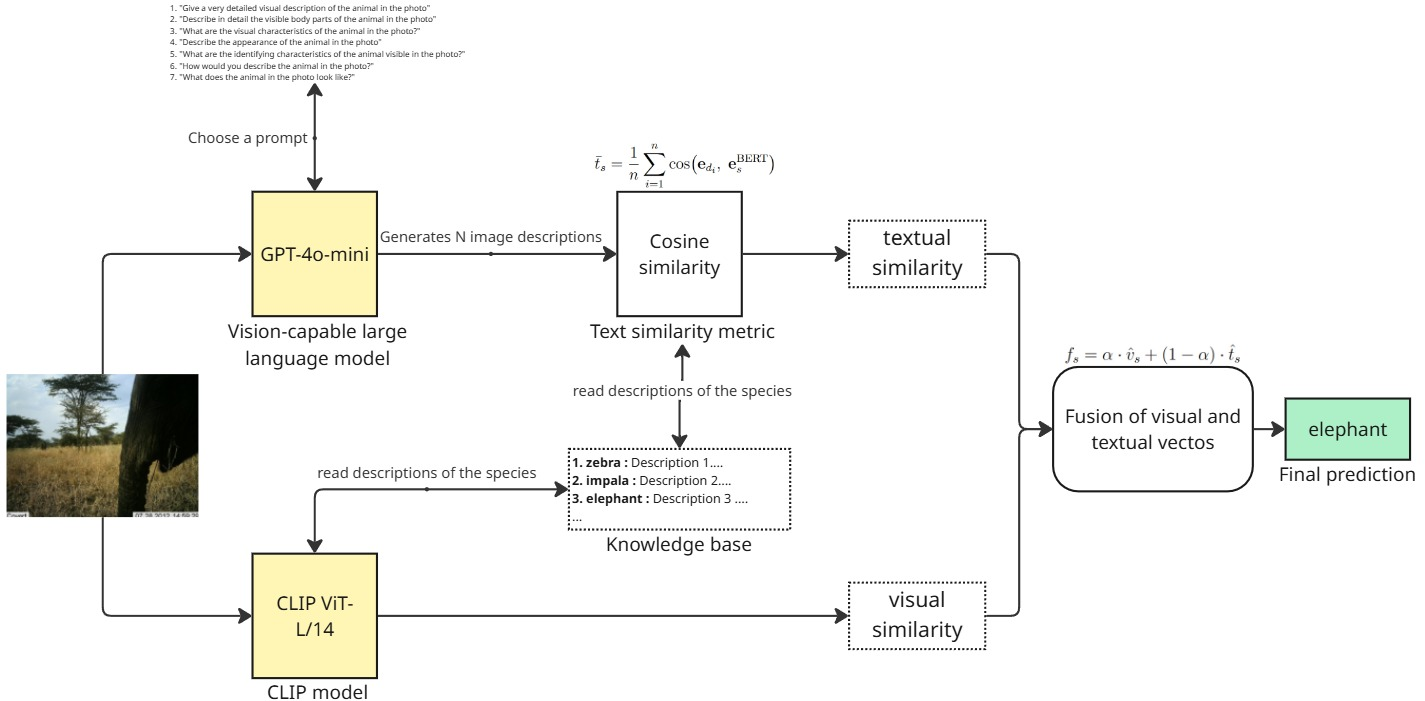
\includegraphics[width=6in]{images/clip_fusion.png}
\caption{WildMatch-CLIP-LLM-Fusion architecture}
\label{fig:clip_fusion}
\end{figure*}

The pipeline takes two inputs for each prediction: a camera trap image and a pre-built knowledge base. Two image variants are considered in the evaluation: full-frame images and cropped images, where the latter correspond to regions containing the animal as obtained through an animal detection step. The knowledge base is represented as a structured JSON resource mapping each candidate species name to a set of textual fields. The key element used during inference is the \textit{Visually Relevant Summary} (VRS), defined as a paragraph-length description of the species' visible appearance. These summaries are generated offline by prompting GPT-4o-mini to extract only photographically observable information from the corresponding Wikipedia article, while excluding non-visual attributes (e.g., measurements, sounds, and smells) and returning a single paragraph.

The experiments are conducted on three camera-trap datasets (Caltech, Serengeti, and WCS). For each dataset, classification is performed over a fixed candidate set corresponding to the species available in that dataset subset. The same candidate set is used to define the class labels and to construct the species entries in the knowledge base used during inference.

\begin{itemize}
\item \textbf{Serengeti (12 species, common names):} zebra, hyenaspotted, warthog, impala, elephant, giraffe, buffalo, guineafowl, ostrich, cheetah, hippopotamus, baboon.
\item \textbf{WCS (10 species, scientific names):} \textit{Equus quagga}, \textit{Bos taurus}, \textit{Loxodonta africana}, \textit{Mitu tuberosum}, \textit{Macaca nemestrina}, \textit{Tapirus terrestris}, \textit{Argusianus argus}, \textit{Psophia leucoptera}, \textit{Panthera onca}, \textit{Hystrix brachyura}.
\item \textbf{Caltech (10 species, common names):} raccoon, coyote, deer, rabbit, bobcat, bird, squirrel, rodent, skunk, lizard.
\end{itemize}

Image preprocessing is minimal and delegated to the CLIP preprocessing transform. The input image is resized, centre-cropped, and normalised according to the model's expected input distribution. No additional augmentation, denoising, or domain-specific preprocessing is applied. The image is loaded and converted to RGB before being passed to the visual encoder.

\subsection{Multimodal Inference Method}

The pipeline consists of three main components: a vision-language model for caption generation, a CLIP-based visual matching branch, and a ModernBERT-based textual matching branch.

A vision-capable large language model, GPT-4o-mini, is used to generate natural-language descriptions of the input image. Rather than relying on a single fixed instruction, the system samples one prompt from a set of paraphrased variants, all aimed at eliciting a detailed visual description of the animal in the photo. This prompt randomisation is intended to encourage descriptive diversity when multiple captions are requested. Each caption is generated with a maximum budget of 500 tokens. In the evaluated configuration, three captions are generated for each image.

The visual branch uses the pre-trained CLIP ViT-L/14 model. CLIP projects both images and texts into a shared 768-dimensional embedding space, allowing similarity computation between the input image and textual species descriptions. Let $\mathbf{e}_{\text{img}}$ denote the $\ell_2$-normalised embedding of the input image. Each species summary from the knowledge base is prepended with a generic camera-trap prompt and encoded through CLIP's text encoder. These text embeddings are computed once and cached for subsequent reuse. For each candidate species $s$, the visual similarity score is defined as the cosine similarity between the image embedding and the cached CLIP text embedding for that species:
\begin{equation}
v_s = \cos\bigl(\mathbf{e}_{\text{img}},\; \mathbf{e}^{\text{CLIP}}_s\bigr).
\end{equation}
This score quantifies the alignment between the visual content of the image and the species-specific textual description represented in the CLIP embedding space.

The textual branch uses \texttt{answerdotai/ModernBERT-base} model. To obtain fixed-length sentence representations, the last hidden state is mean-pooled across all tokens and then $\ell_2$-normalised. Each caption generated by the vision-language model is encoded into a ModernBERT embedding. Similarly, each VRS in the knowledge base is encoded and cached. For each caption $d_i$, cosine similarity is computed against all species embeddings. If $n$ captions are generated, the per-species textual score is obtained by averaging the cosine similarities across captions:
\begin{equation}
\bar{t}_s = \frac{1}{n}\sum_{i=1}^{n}\cos\bigl(\mathbf{e}_{d_i},\; \mathbf{e}^{\text{BERT}}_s\bigr).
\end{equation}
After averaging, the textual score vector is min--max normalised to the interval $[0,1]$.

The final species ranking is obtained by combining the visual and textual score vectors through a weighted linear fusion. When score normalisation is enabled, both the CLIP visual scores and the ModernBERT textual scores are independently min--max normalised to $[0,1]$. The fused score for species $s$ is then computed as:
\begin{equation}
f_s = \alpha \cdot \hat{v}_s + (1-\alpha)\cdot \hat{t}_s,
\end{equation}
where $\hat{v}_s$ and $\hat{t}_s$ are the normalised visual and textual scores, respectively, and $\alpha \in [0,1]$ controls the contribution of each modality. In the evaluated configuration, $\alpha = 0.7$, assigning 70\% of the final score to the CLIP visual branch and 30\% to the textual branch. The predicted label is the species associated with the maximum fused score:
\begin{equation}
\hat{y} = \arg\max_s f_s.
\end{equation}

In addition to the predicted label, the method outputs a confidence value based on the relative margin between the two highest fused scores. Let $f_{(1)}$ and $f_{(2)}$ denote the highest and second-highest fused scores, respectively. The confidence is defined as:
\begin{equation}
c = \frac{f_{(1)}}{f_{(1)} + f_{(2)}}.
\end{equation}
This formulation yields values in the interval $(0.5, 1]$. Scores close to 1 indicate a large separation between the top-ranked and second-ranked candidates, whereas a value near 0.5 corresponds to a near tie.

For each test image, the inference process follows five steps:
\begin{enumerate}
\item The vision-language model generates $n$ captions for the input image.
\item The image is encoded with CLIP, and cosine similarities are computed against the cached CLIP text embeddings of all candidate species.
\item Each generated caption is encoded with ModernBERT, cosine similarities are computed against the cached textual embeddings of all species, and the resulting scores are averaged across captions and normalised.
\item The visual and textual score vectors are independently normalised and fused through the weighted linear combination defined above.
\item The species with the highest fused score is returned as the final prediction together with the confidence estimate.
\end{enumerate}

\subsection{Experimental Protocol and Configuration}

No training, fine-tuning, or parameter optimisation is performed in the evaluated system. CLIP ViT-L/14, ModernBERT-base, and GPT-4o-mini are used with their original pre-trained parameters. The fusion weight $\alpha$ is fixed rather than learned. The construction of the knowledge base is executed as an offline preprocessing step and does not involve gradient-based learning. Accordingly, the complete method operates in a zero-shot regime with respect to the target species classification task.

Evaluation is conducted on the full set of available images for each dataset configuration. No train/test split is performed. The primary metric is top-1 classification accuracy, computed as the proportion of images for which the predicted species matches the ground-truth label. For each image, the system records the true label, predicted label, confidence score, and modality-specific scores for subsequent analysis. The reported experimental results compare the proposed CLIP Fusion approach against a baseline across three datasets---Caltech, Serengeti, and WCS---and under two image settings, namely cropped and full-frame images.

The evaluated configuration uses the following settings:
\begin{itemize}
\item CLIP model: ViT-L/14;
\item text encoder: ModernBERT-base;
\item vision-language model for caption generation: GPT-4o-mini;
\item number of captions per image: $n=3$;
\item fusion weight: $\alpha = 0.7$;
\item score normalisation: min--max scaling to $[0,1]$;
\item CLIP text prompt: a generic camera-trap prefix applied to species summaries;
\item caption generation temperature: 0.7 when $n>1$;
\item maximum caption length: 500 tokens.
\end{itemize}

\section{Experiments and Results}

\subsection{Results Across Datasets and Image Settings}

The experiments evaluate the behaviour of the proposed multimodal pipeline across six principal configurations formed by the combination of three datasets (Caltech, Serengeti, and WCS) and two image types (cropped and full). For each configuration, results are reported for the baseline approach and for the CLIP Fusion pipeline. The main quantities reported are classification accuracy, average confidence, total number of evaluated samples, and number of correct predictions. The comparison between baseline and CLIP Fusion is further summarised in terms of absolute accuracy improvement and change in average confidence.

Table~\ref{tab:exp02_accuracy_summary} summarises the top-1 accuracy results for the six evaluated dataset--image configurations. The proposed CLIP Fusion method outperformed the baseline in four of the six configurations (Caltech cropped, Serengeti cropped, WCS cropped, and WCS full), while slight decreases were observed for Caltech full and Serengeti full.

\begin{table}[t]
\centering
\caption{Top-1 accuracy and number of correct predictions for the baseline and the proposed CLIP Fusion pipeline across datasets and image settings.}
\label{tab:exp02_accuracy_summary}
\resizebox{\textwidth}{!}{%
\begin{tabular}{l l r c c c r r}
\hline
\textbf{Dataset} & \textbf{Image} & \textbf{Samples} & \textbf{Acc. (Base)} & \textbf{Acc. (Fusion)} & \textbf{$\Delta$Acc. (pp)} & \textbf{Correct (Base)} & \textbf{Correct (Fusion)} \\
\hline
Caltech & Cropped & 1000 & 68.3\% & 73.5\% & +5.20 & 683 & 735 \\
Caltech & Full & 1000 & 58.1\% & 58.0\% & $-0.10$ & 581 & 580 \\
Serengeti & Cropped & 1200 & 67.0\% & 68.75\% & +1.75 & 804 & 825 \\
Serengeti & Full & 1200 & 66.42\% & 65.25\% & $-1.17$ & 797 & 783 \\
WCS & Cropped & 1000 & 58.2\% & 60.7\% & +2.50 & 582 & 607 \\
WCS & Full & 1000 & 72.1\% & 76.4\% & +4.30 & 721 & 764 \\
\hline
\end{tabular}%
}
\end{table}

The absolute accuracy improvements of CLIP Fusion relative to the baseline (Table~\ref{tab:exp02_accuracy_summary}) ranged from $-1.17$ to +5.20 percentage points. Across all six configurations, the average reported improvement was 2.08 percentage points. The largest improvement was obtained for Caltech cropped images (+5.20 pp), while the largest decrease relative to baseline occurred for Serengeti full images ($-1.17$ pp). Table~\ref{tab:exp02_accuracy_summary} also reports the sample counts and the absolute numbers of correct predictions. The most pronounced gains in absolute numbers of correctly classified images were obtained for Caltech cropped (from 683 to 735 correct predictions) and WCS full (from 721 to 764).

\subsection{Confidence Analysis}

Average confidence increased for CLIP Fusion in all reported baseline comparisons, regardless of whether accuracy improved (Table~\ref{tab:exp02_confidence_summary}). The corresponding confidence changes ranged from +7.83 to +11.40 percentage points. The largest increase in average confidence was observed for Caltech full images, even though this configuration did not improve in terms of classification accuracy.

\begin{table}[t]
\centering
\caption{Average confidence for the baseline and the proposed CLIP Fusion pipeline across datasets and image settings.}
\label{tab:exp02_confidence_summary}
\begin{tabular}{l l c c}
\hline
\textbf{Dataset} & \textbf{Image} & \textbf{Conf. (Base)} & \textbf{Conf. (Fusion)} \\
\hline
Caltech & Cropped & 86.87\% & 96.50\% \\
Caltech & Full & 84.00\% & 95.40\% \\
Serengeti & Cropped & 88.78\% & 96.69\% \\
Serengeti & Full & 86.50\% & 96.06\% \\
WCS & Cropped & 88.07\% & 96.80\% \\
WCS & Full & 87.83\% & 95.67\% \\
\hline
\end{tabular}
\end{table}

\section{Discussion}

The reported results indicate that the integration of CLIP-based visual matching and language-model-assisted textual matching can improve zero-shot species classification performance in several camera trap scenarios. In particular, the proposed fusion strategy achieved higher top-1 accuracy in four of the six main evaluated configurations, with gains ranging from 1.75 to 5.20 percentage points. The largest positive effects were observed for cropped images in Caltech and for full images in WCS.

At the same time, the results do not indicate uniform improvement across all settings. In full-image configurations for Caltech and Serengeti, the baseline slightly outperformed the proposed fusion approach. This outcome suggests that the contribution of the additional textual branch and the weighted fusion mechanism is dependent on the dataset and image setting under evaluation. Based on the reported experiments alone, the method should therefore be interpreted as beneficial in several, but not all, tested conditions.

The confidence analysis shows a consistent increase in average confidence for CLIP Fusion across all six baseline comparisons. However, these increases in confidence do not always coincide with higher classification accuracy. This is evident in the Caltech full and Serengeti full settings, where CLIP Fusion produced higher average confidence despite lower accuracy than the baseline. Therefore, within the reported experimental evidence, confidence values derived from the fused-score margin appear to reflect score separation between top-ranked classes, but not necessarily improved correctness in every configuration.

The results also illustrate the effect of combining complementary modalities without task-specific training. The visual branch directly compares the input image with species descriptions in CLIP space, while the textual branch introduces an intermediate image description generated by a vision-language model and matched against species summaries with ModernBERT. The observed improvements in four configurations support the view that these two branches can provide complementary information under zero-shot inference. Nevertheless, the reported results do not isolate the independent contribution of each component beyond the comparison to the baseline and the aggregate fusion outcomes.

Some limitations are explicitly identifiable from the described implementation and evaluation protocol. First, the pipeline performs no train/test split and evaluates on all available images. Consequently, the reported results are limited to this evaluation setup and do not include an analysis of generalisation under separate training and testing partitions. Second, the ModernBERT representations are obtained by mean-pooling token embeddings rather than using a dedicated sentence-embedding model, which may be suboptimal for semantic similarity. Third, the method depends on an offline-generated knowledge base whose visually relevant summaries are derived from Wikipedia through GPT-4o-mini prompting. The reported text does not provide an independent evaluation of the effect of summary quality on final classification performance.

A further point concerns the mechanism used for multiple captions. Although the implementation name suggests a voting procedure, the actual method averages textual similarity scores across captions before fusion. This distinction is relevant for interpreting the behaviour of the system, because the reported results correspond to score aggregation rather than label-level majority voting.

Overall, the experiment supports the feasibility of a training-free multimodal classification pipeline for camera trap species recognition. The evidence provided by the reported results shows that this approach can improve top-1 accuracy in several configurations while maintaining a consistent increase in average confidence, although the gains are not universal across all datasets and image types.

\section{Final Remarks}

This chapter described a zero-shot multimodal experiment for species classification in camera trap images based on the \textit{WildMatch-CLIP-LLM-Fusion} pipeline. The method combines a CLIP-derived visual similarity signal with a textual similarity signal obtained from GPT-4o-mini image descriptions and ModernBERT-based semantic matching against species summaries stored in a knowledge base. Final predictions are produced through weighted linear fusion, with no training or fine-tuning performed for the target task.

The reported evaluation showed that the fusion strategy improved top-1 accuracy in four out of six baseline comparisons, with an average gain of 2.08 percentage points across the evaluated configurations. The strongest improvements were observed for Caltech cropped images and WCS full images, while slight performance decreases were observed in two full-image settings. Average confidence increased in all comparisons, although these increases did not always correspond to higher accuracy.

Within the context of this thesis, the experiment contributes a concrete example of how multimodal pre-trained models can be integrated into camera trap workflows without requiring task-specific model training. The results indicate that such integration can be effective under several zero-shot evaluation settings, while also highlighting limitations related to dataset dependence, confidence interpretation, encoder choice, and evaluation protocol.
\chapter{Project Proceedings}\label{cap:conclusion}

In this thesis proposal, we highlight that despite significant advancements in
image classification, real-world applications like species classification in
camera-trap images still face many challenges. These challenges need to be
addressed to ensure that the data extracted using fully automated AI-based
systems is reliable for use in ecological studies. We presented solutions to
specific challenges to improve classification performance, directly impacting
tasks such as filtering empty camera-trap images, species classification, and
counting individuals. In Section~\ref{sec:contrib}, we present the contributions
of this work, and in Section~\ref{sec:sched}, we outline the next steps of the
research and the schedule.

\section{Contributions}\label{sec:contrib}

The contributions of this work are primarily based on the improvement of
classification models and can be divided according to three tasks in automatic
information extraction from camera-trap images: filtering empty images, species
classification, and counting individuals.

For the task of filtering empty images, we presented a comparative study to
analyze the trade-off between precision and inference latency of classification
and detection models when the inference is done directly on edge devices.
Although some studies have addressed this matter, they typically use small
datasets with a limited number of species, which restricts the scope of their
conclusions. Our work, however, utilizes two large-scale camera-trap datasets to
assess this trade-off more comprehensively. We also applied a series of model
optimizations to reduce inference latency and compared their impact on model
precision. We found that detectors generally outperform classifiers with
comparable inference latency; however, classifiers can achieve higher
performance on this task if a larger amount of labeled images is available,
which is more challenging to obtain for detectors. Another finding is that
models with higher input resolution perform better at filtering empty images,
and their inference latency can be kept competitive by reducing the number of
model filters.

For the widely studied task of species identification, we addressed the problem
of long-tail classification, which is often neglected in works on camera-trap
image species classification, with tail classes typically being removed or
grouped into generic categories. Our main contribution in this area is the
introduction of a new framework called Square-root Sampling Branch (SSB). This
framework employs a multi-branch network combined with sampling strategies to
enhance performance on tail classes while maintaining minimal loss in head
classes' accuracy compared to state-of-the-art long-tail methods. Additionally,
we provide strong classification baselines on four large-scale camera-trap
datasets using the latest training tricks.

For the task of counting animals, we followed the formulation proposed by the
iWildCam 2021 benchmark, where the training set does not contain labels for
counting, necessitating unsupervised learning. Our main contribution was the
development of a strong baseline comprising an ensemble of classifiers
supplemented with counting heuristics based on bounding boxes generated by
object detector models. Our solution won the iWildCam 2021 competition, held at
The Eighth Workshop on Fine-Grained Visual Categorization (FGVC8) during CVPR
2021. Although we explored various methods to obtain more reliable counting
results, such as multi-object tracking and re-identification models based on
bounding boxes, they yielded inferior results compared to our heuristic-based
approach. This highlights the complexity of the problem. In this task, we still
aim to improve the classification subtask by applying the other improvements
proposed in this work.

\section{Next Steps and Schedule}\label{sec:sched}

The next steps of this research will include developing strategies for the 
classification of capture events, applying all classification innovations proposed in
this work to improve the task of counting the number of animals of each species,
and writing the final thesis. \autoref{tab:schedule} shows the schedule of the
activities described as follows:

\begin{itemize}
\item \textbf{A01 - Multi-image experiments}: Develop strategies to improve
species identification based on a sequence of images of the same individual.

\item \textbf{A02 - Multi-image results analysis}: Analyze the results obtained
during the multi-image experiments.

\item \textbf{A03 - Multi-image approach paper}: Write a scientific paper
reporting our proposed multi-image strategies for species classification using a
sequence of images.

\item \textbf{B01 - Improve counting animals task}: Apply all classification
innovations proposed in this work to improve the task of counting the number of
animals of each species.

\item \textbf{B02 - Counting animals results analysis}: Analyze the results on
the task of classifying species and counting individual animals present in a
sequence of images.

\item \textbf{C01 - Thesis writing}: Write the final thesis.

\item \textbf{C02 - Thesis defense}
\end{itemize}



\begin{table}[h]
\centering
\caption{Research schedule by month}
\label{tab:schedule}
\begin{tabular}{|c|lllllll|}
\hline
\multicolumn{1}{|c|}{} &
  \multicolumn{7}{c|}{2025} \\ \cline{2-8}
\multicolumn{1}{|c|}{\multirow{-2}{*}{Activities}} &
  \multicolumn{1}{c|}{Jun} &
  \multicolumn{1}{c|}{Jul} &
  \multicolumn{1}{c|}{Ago} &
  \multicolumn{1}{c|}{Sep} &
  \multicolumn{1}{c|}{Oct} &
  \multicolumn{1}{c|}{Nov} &
  \multicolumn{1}{c|}{Dec} \\ \hline
A01 &
  \multicolumn{1}{l|}{\cellcolor[HTML]{9B9B9B}{\color[HTML]{330001} }} &
  \multicolumn{1}{l|}{\cellcolor[HTML]{9B9B9B}{\color[HTML]{330001} }} &
  \multicolumn{1}{l|}{} &
  \multicolumn{1}{l|}{} &
  \multicolumn{1}{l|}{} &
  \multicolumn{1}{l|}{} &
   \\ \hline
A02 &
  \multicolumn{1}{l|}{} &
  \multicolumn{1}{l|}{\cellcolor[HTML]{9B9B9B}} &
  \multicolumn{1}{l|}{} &
  \multicolumn{1}{l|}{} &
  \multicolumn{1}{l|}{} &
  \multicolumn{1}{l|}{} &
   \\ \hline
A03 &
  \multicolumn{1}{l|}{} &
  \multicolumn{1}{l|}{\cellcolor[HTML]{9B9B9B}} &
  \multicolumn{1}{l|}{\cellcolor[HTML]{9B9B9B}} &
  \multicolumn{1}{l|}{\cellcolor[HTML]{9B9B9B}} &
  \multicolumn{1}{l|}{} &
  \multicolumn{1}{l|}{} &
   \\ \hline
B01 &
  \multicolumn{1}{l|}{} &
  \multicolumn{1}{l|}{} &
  \multicolumn{1}{l|}{} &
  \multicolumn{1}{l|}{\cellcolor[HTML]{9B9B9B}} &
  \multicolumn{1}{l|}{} &
  \multicolumn{1}{l|}{} &
   \\ \hline
B02 &
  \multicolumn{1}{l|}{} &
  \multicolumn{1}{l|}{} &
  \multicolumn{1}{l|}{} &
  \multicolumn{1}{l|}{} &
  \multicolumn{1}{l|}{\cellcolor[HTML]{9B9B9B}} &
  \multicolumn{1}{l|}{} &
   \\ \hline
C01 &
  \multicolumn{1}{l|}{} &
  \multicolumn{1}{l|}{} &
  \multicolumn{1}{l|}{} &
  \multicolumn{1}{l|}{\cellcolor[HTML]{9B9B9B}} &
  \multicolumn{1}{l|}{\cellcolor[HTML]{9B9B9B}} &
  \multicolumn{1}{l|}{\cellcolor[HTML]{9B9B9B}} & 
  \multicolumn{1}{l|}{} \\ \hline
C02 &
  \multicolumn{1}{l|}{} &
  \multicolumn{1}{l|}{} &
  \multicolumn{1}{l|}{} &
  \multicolumn{1}{l|}{} &
  \multicolumn{1}{l|}{} &
  \multicolumn{1}{l|}{} &
  \multicolumn{1}{l|}{\cellcolor[HTML]{9B9B9B}} \\ \hline
\end{tabular}
\end{table}


\ppgccbibliography{base}

\end{document}
